\newline

\paragraph{Plan du document:} La section~\ref{section-VEF-am\'eliorations} pr\'esente le Lot 1, qui concentre des axes d'am\'elioration de l'existant.
Les travaux concernant les mod\`eles de turbulence font l'objet du Lot 2 et sont d\'ecrits dans la section~\ref{section-turbulence}.
La section qui suit concerne le d\'eveloppement des nouveaux sch\'emas num\'eriques de discr\'etisation en espace, \`a savoir un sch\'ema de type Galerkin Discontinu (section~\ref{section-GD}, Lot 3.1) ainsi que le d\'eveloppement d'un mod\`ele fin pour les assemblages combustibles (section~\ref{section-poreux}, Lot 3.2).
La section~\ref{dd_qi}, est d\'edi\'ee aux travaux concernant l'estimateur d'erreurs {\it{a posteriori}} (section~\ref{section-estimateurs-erreurs}, Lot 4.1),  la d\'ecomposition de domaine (section~\ref{section-DD}, Lot 4.2) ainsi que la quantification des incertitudes (section~\ref{section-QI}, Lot 4.3) . 
Le lot 5 est consacr\'e \`a la mise en {\oe}uvre de nouvelles fonctionnalit\'es, avec une composante ALE pour la r\'ealisation de calculs d'interaction fluide-structure (section~\ref{section-ALE}, Lot 5.1), un mod\`ele compressible (section~\ref{section-compressible}, Lot 5.2), la mod\'elisation polydisperse de particules solides (section~\ref{section-polydisperse}, Lot 5.3) et le couplage avec une librairie de transport chimique (section~\ref{section-scorpio}, Lot 5.4). Enfin, le travail de validation et de documentation \`a r\'ealiser en continu est d\'ecrit dans la section~\ref{section-vvdoc}, Lot 6.


% VEF VEF VEF VEF VEF VEF VEF VEF VEF VEF VEF VEF VEF VEF VEF VEF VEF VEF
% VEF VEF VEF VEF VEF VEF VEF VEF VEF VEF VEF VEF VEF VEF VEF VEF VEF VEF

\section{\'evolutions des sch\'emas et techniques existants }
\label{section-VEF-am\'eliorations}
\subsection{Compressibilit\'e artificielle}
\label{Algo-Stat}
Dans TrioCFD, les solutions stationnaires sont calcul\'ees via la r\'esolution d'un transitoire. Cette phase instationnaire est dans certains cas tr\`es co\^uteuse en temps CPU. 

L'approche multi-pas implique la r\'esolution d'une \'equation de Poisson pour la pression (l'\'etape $2$) \`a chaque pas de temps, ce qui peut s'av\'erer tr\`es co\^uteux en temps de calcul. Afin de s'affranchir de la r\'esolution de l'\'equation de Poisson pour la pression, une m\'ethode de type compressibilit\'e artificielle est envisageable.
L'id\'ee de la m\'ethode consiste \`a introduire un param\`etre de "p\'enalisation" $\epsilon$ et \`a remplacer la contrainte $\nabla. \velocity = 0$ par:

$$\epsilon \frac{\partial p}{\partial t} + \nabla. \velocity = 0 .$$

La contrainte d'incompressibilit\'e est satisfaite seulement \`a la convergence. 
Le param\`etre $\epsilon$ est arbitraire.  Il doit \^etre choisi de mani\`ere optimale  afin d'assurer une convergence rapide mais \'egalement \`a assurer l'existence d'une solution
num\'erique stationnaire.


Ainsi, (\ref{schema-implicit}) s'\'ecrit:

\begin{itemize}
\itemb  
{\bf{Etape 1~:}}
$$ \ds{\left( \frac{1}{\Delta t} M - A + L(U^n) -  \frac{\Delta t}{\epsilon} B^TM^{-1}B \right) U^{n+1}  = \frac{1}{\Delta t} M U^n - B^T P^n + S^n,}$$ 
\itemb
{\bf{Etape 2~:}}
$$ \ds{P^{n+1} = P^n  - \frac{\Delta t}{\epsilon} M^{-1}B U^{n+1}.} $$
\end{itemize}

C'est une discr\'etisation \`a l'ordre $1$ en temps mais comme on s'int\'eresse \`a l'obtention d'un \'etat stationnaire cela ne pose pas de probl\`eme de pr\'ecision. N\'eanmoins, une g\'en\'eralisation de la m\'ethode permettant de monter en ordre est propos\'ee dans l'article~\cite{guermond2015high} .


\begin{center}
\begin{longtable}{|l|l|} 
\hline
\rowcolor{couleur1}\multicolumn{2}{|c|}{Lot 1~: \'evolutions de l'existant}\\
\rowcolor{couleur2}\multicolumn{2}{|c|}{Sous-Lot 1.1~: compressibilit\'e artificielle}\\
%\rowcolor{couleur3}\multicolumn{2}{|c|}{T\^ache 1.1.a~:  compressibilit\'e artificielle}\\
\hline Objectif & d\'eveloppement d'un algorithme stationnaire efficace.\\
\hline R\'ef\'erences &  \cite{guermond2015high} et autres \`a d\'efinir \\
\hline T\^aches \`a r\'ealiser & impl\'ementation dans TrioCFD et validation \\
\hline Risques identifi\'es & - m\'ethode de r\'esolution diff\'erente de celle de TrioCFD~; \\
 &- impl\'ementation informatique cons\'equente ; \\
\hline Conditionnement de l'action & aucun \\
\hline Charge de travail & D\'eveloppement et R\&D court terme \\
\hline
\end{longtable}
\end{center}


\begin{rque}
 
Des r\'eflexions sur le d\'eveloppement de la m\'ethode de compressibilit\'e artificielle ont eu lieu. La mise en {\oe}uvre dans TrioCFD peut se faire sans un impact majeur sur les autres parties du code, la difficult\'e r\'eside dans le fait que c'est une m\'ethode de r\'esolution diff\'erente de celle de TrioCFD. 
\end{rque}

\subsection{Am\'elioration de la stabilit\'e du sch\'ema VEF}
\label{Progres-VEF}

La m\'ethode VEF permet une discr\'etisation polynomiale d'ordre $1$ avantageuse du probl\`eme de Stokes, car la matrice de masse de la vitesse est diagonale. Mais si on se contente d'une pression $P_0$, ce sch\'ema manque de pr\'ecision lorsque le terme  source de l'\'equation de quantit\'e de mouvement est raide \cite{Emon92}. Une analyse math\'ematique montre que ce probl\`eme est li\'e \`a la dimension de l'espace des vitesses, trop grande par rapport \`a celle de l'espace des pression. Pour am\'eliorer la pr\'ecision du sch\'ema de base, il a donc \'et\'e propos\'e dans \cite{Heib03} pour le $2D$ et \cite{Fort06} pour le $3D$ d'augmenter le nombre de degr\'es de libert\'e en pression. Cette technique est efficace mais fait augmenter le nombre d'inconnues, ce qui peut \^etre p\'enalisant pour passer de gros cas-tests. Il existe des m\'ethodes alternatives (en gardant une pression $P_0$) pour obtenir une bonne approximation d'ordre $1$ du champ de vitesse \`a divergence nulle~:
%-------------%
\begin{itemize}
\item En utilisant les \'el\'ements finis de Crouzeix-Raviart non conformes et en projetant la vitesse discr\`ete sur un espace appropri\'e (Linke et al \cite{Link14,JKMN17}).
\item En r\'eduisant alg\'ebriquement l'espace des vitesses \cite{Hech81}.
\item En utilisant les \'el\'ements finis de Taylor-Hood d'ordre $1$  stabilis\'es, tels que $(\velocity_h,p_h)\in\vec{P}_1\times P_0$, et post-trait\'es \cite{BaVa10,AlBN18}. 
\end{itemize}
%-----------%
Dans \cite{GLRW12}, les auteurs montrent qu'il est crucial d'approcher pr\'ecisement l'espace des vitesses \`a divergence nulle, en particulier dans les cas o\`u le terme  source de l'\'equation de quantit\'e de mouvement est raide. Il est donc important de poursuivre les travaux en cours concernant la recherche d'un sch\'ema d'ordre $1$ pr\'ecis et peu gourmand en nombre d'inconnues.
%--------------------------------%
\subsubsection{M\'ethode de projection}
%--------------------------------%
R\'ecemment, Linke et al \cite{Link14,JKMN17} ont propos\'e d'utiliser des m\'ethodes de projection pour supprimer les vitesses parasites. La m\'ethode de projection sur l'espace des \'el\'ements finis de Raviart-Thomas \cite{RaTh77} a \'et\'e \'evolu\'ee dans la version 1.7.8, et pr\'esente des r\'esultats int\'eressants \cite{Jame18}. Actuellement, cette m\'ethode est fonctionnelle dans TrioCFD dans le cas stationnaire, avec des conditions aux limites de Dirichlet. Notons que la projection sur les \'el\'ements finis de Raviart-Thomas ne permet pas de traiter les sch\'emas explicites en temps car la matrice de masse projet\'ee n'est pas de rang maximal. Pour cela, il faut impl\'ementer la projection sur les \'el\'ements finis de Brezzi-Douglas-Marini \cite{BrDM85} (les BDM). La matrice de masse projet\'ee sera alors de rang maximal, mais elle ne sera pas diagonale. Ceci implique qu'on a besoin d'un solveur de pression (de la forme $BM^{-1}B^T$) g\'en\'eral pour lequel la matrice de masse ne soit pas n\'ecessairement diagonale. Il faut donc poursuivre la phase d'industrialisation.
%------------%
\begin{center}
\begin{longtable}{|l|l|} 
\hline
\rowcolor{couleur1}\multicolumn{2}{|c|}{Lot 1~: \'evolutions de l'existant}\\
\rowcolor{couleur2}\multicolumn{2}{|c|}{Sous-Lot 1.2~: Am\'elioration de la stabilit\'e du sch\'ema VEF }\\
\rowcolor{couleur3}\multicolumn{2}{|c|}{T\^ache 1.2.a~: M\'ethode de projection}
\\
\hline 
Objectif & Industrialiser la m\'ethode de projection.
\\
\hline
Etapes & Mettre \`a jour les d\'eveloppements.
       \\
       & Coder le traitement de toutes les conditions limites.
       \\
       & Inclure dans le sch\'ema la projection de la matrice de masse.
       \\
       & Tester diff\'erents sch\'emas de discr\'etisation de la convection.
       \\
       & Appliquer la projection sur les BDM.
       \\
       & Traiter le sch\'ema explicite en temps.
       \\
\hline 
R\'ef\'erences & Linke et al \cite{Link14,JKMN17}
\\
\hline Risques & travail de recherche, complexit\'e de la mise en {\oe}uvre informatique dans un code existant\\
\hline Pr\'erequis & Solveur de pression g\'en\'eral pour traiter le cas explicite \\
\hline Charge de travail & R\&D moyen terme: action en cours\\
\hline
\end{longtable}
\end{center}
%----------%
%---------------------------------------------%
\subsubsection{M\'ethode d'\'elimination des vitesses}
%---------------------------------------------%
Dans l'article \cite{Hech81}, Hecht propose un algorithme pour construire une base de fonctions $\vec{P}_1^{NC}$ \`a divergence nulle. La m\'ethode utilise des r\'esultats de la th\'eorie des graphes sur les arbres maximaux et le r\'esultat final semble simple \`a programmer. On peut r\'esoudre le probl\`eme de Stokes en \'eliminant la variable de pression, ce qui rend inutile dans ce cas l'algorithme pr\'ediction-correction. Il serait int\'eressant de tester l'efficacit\'e de m\'ethode, et de d\'eterminer si elle est compatible avec le parall\'elisme du code actuel.
%------------%
\begin{center}
\begin{longtable}{|l|l|} 
\hline
\rowcolor{couleur1}\multicolumn{2}{|c|}{Lot 1~: \'evolutions de l'existant}\\
\rowcolor{couleur2}\multicolumn{2}{|c|}{Sous-Lot 1.2~: Am\'elioration de la stabilit\'e du sch\'ema VEF }\\
\rowcolor{couleur3}\multicolumn{2}{|c|}{T\^ache 1.2.b~: M\'ethode d'\'elimination des vitesses}
\\
\hline 
Objectif & Evaluer l'int\'er\^et de la m\'ethode.
\\
\hline
Etapes & Impl\'ementer et tester la m\'ethode dans une maquette.
       \\
       & Stokes $2D$ puis $3D$ puis Oseen puis Navier-Stokes.
       \\
       & Etudier l'int\'egration dans TrioCFD.
       \\
       & D\'ecider de l'industrialisation.
       \\
\hline 
R\'ef\'erences & Hecht \cite{Hech81}
\\
\hline Risques & travail de recherche, complexit\'e de la mise en {\oe}uvre informatique dans un code existant\\
\hline Pr\'erequis & Architecture de code souple et Lot 1.2.a achev\'e. \\
\hline Charge de travail & R\&D court terme.\\
\hline
\end{longtable}
\end{center}
%----------%
%----------------------------------------------------------%
\subsubsection{El\'ements finis $\vec{P}_1\times P_0$ stabilis\'es}
%----------------------------------------------------------%
Il est connu que les \'el\'ements finis de Taylor-Hood d'ordre $1$, tels que $(\velocity_h,p_h)\in\vec{P}_1\times P_0$, ne sont pas stables car le nombre de simplexes devient rapidement plus important que la dimension multipli\'ee par le nombre de sommets. Cependant, on peut stabiliser le syst\`eme lin\'eaire en ajoutant \`a la contrainte de divergence nulle un terme de p\'enalisation des sauts de pression. Cette m\'ethode est particuli\`erement \'econome en nombre d'inconnues. De plus la matrice de masse $P_1$ est \'equivalente \`a une matrice diagonale. Dans \cite{BaVa10,AlBN18}, les auteurs proposent de calculer un rel\`evement des sauts de pression avec les \'el\'ements finis de Raviart-Thomas pour reconstruire un champ de vitesse \`a divergence nulle ponctuelle. Cette m\'ethode est \`a mettre en concurrence avec les deux autres m\'ethodes cit\'ees pr\'ec\'edemment. C'est \`a ce jour la m\'ethode la plus \'econome en nombre d'inconnues pour r\'esoudre le probl\`eme de Stokes sur maillage de simplexes.
%------------%
\begin{center}
\begin{longtable}{|l|l|} 
\hline
\rowcolor{couleur1}\multicolumn{2}{|c|}{Lot 1~: \'evolutions de l'existant}\\
\rowcolor{couleur2}\multicolumn{2}{|c|}{Sous-Lot 1.2~: Am\'elioration de la stabilit\'e du sch\'ema VEF }\\
\rowcolor{couleur3}\multicolumn{2}{|c|}{T\^ache 1.2.c~: El\'ements finis $\vec{P}_1\times P_0$ stabilis\'es}\\
\hline 
Objectif & Evaluer l'int\'er\^et de la m\'ethode.
\\
\hline
Etapes & Impl\'ementer et tester la m\'ethode dans une maquette.
       \\
       & Stokes $2D$ puis $3D$ puis Osen puis Navier-Stokes.
       \\
       & Etudier l'int\'egration dans TrioCFD.
       \\
       & D\'ecider de l'industrialisation.
       \\
\hline 
R\'ef\'erences & Barranechea et al \cite{BaVa10,AlBN18}
\\
\hline Risques & travail de recherche, complexit\'e de la mise en {\oe}uvre informatique dans un code existant\\
\hline Pr\'erequis & Architecture de code souple et Lot 1.2.a achev\'e. \\
\hline Charge de travail & R\&D court terme.\\
\hline
\end{longtable}
\end{center}

\subsection{Discr\'etisation des termes de convection non lin\'eaire}
\label{section-Skew}

\subsubsection{Revue des discr\'etisations des termes de convection disponibles dans TrioCFD }

On s'int\'eresse aux termes de convection non-lin\'eaire, dont la discr\'etisation agit significativement sur la robustesse des simulations. En effet, les solutions produites par les techniques de discr\'etisation centr\'ees sont instables, et  les m\'ethodes d\'ecentr\'ees  standards conduisent \`a une diffusion num\'erique excessive. Le code TrioCFD dispose d'une dizaine de mot-cl\'es permettant de pr\'eciser le sch\'ema pour les termes de convection. En pratique, trois options sont principalement utilis\'ees ({\sc{amont}}, {\sc{muscl}}, {\sc{EF\_stab}}). Elles sont d\'ecrites en Annexe  (section~\ref{section-annexe-convection}). 

Les \'etudes montrent une tr\`es forte sensibilit\'e des calculs au sch\'ema de convection choisi. \\
Cette action vise \`a revoir ces m\'ethodes de discr\'etisation, les \'eprouver sur des maillages quelconques et des simulations LES,  les am\'eliorer en tirant profit d'une veille bibliographique.

\begin{center}
\begin{longtable}{|l|l|} 
\hline
\rowcolor{couleur1}\multicolumn{2}{|c|}{Lot 1~: \'evolutions de l'existant}\\
\rowcolor{couleur2}\multicolumn{2}{|c|}{Sous-Lot 1.3~:  discr\'etisation des termes  de convection non lin\'eaires}\\
%\rowcolor{couleur3}\multicolumn{2}{|c|}{T\^ache }\\
\hline Objectif & disposer d'un sch\'ema stable pour les termes de convection, dont la dissipation  \\
&  num\'erique est adapt\'ee aux calculs LES (c'est \`a dire n\'egligeable par rapport \`a \\
& la dissipation du mod\`ele de sous-maille)\\
\hline R\'ef\'erences & \`a d\'efinir\\
\hline T\^aches \`a r\'ealiser &  -  revoir les m\'ethodes de discr\'etisation disponibles, se les r\'eapproprier ;\\
& - faire des tests sur des \'ecoulements turbulents et avec des maillages quelconques ;\\
&- am\'eliorer  l'existant si n\'ecessaire\\
\hline Conditionnement de l'action & Lot 3.1 achev\'e \\
\hline Risques identifi\'es &  travail de recherche, complexit\'e de la mise en {\oe}uvre informatique dans un code existant \\
\hline Charge de travail & R\&D court terme \\
\hline
\end{longtable}
\end{center}



\subsubsection{Conservation de l'\'energie cin\'etique}

Il est \'etabli depuis longtemps que  des temps d'int\'egration longs des termes de convection non lin\'eaires conduisent \`a l'arr\^et des simulations num\'eriques en raison de l'amplification d'instabilit\'es num\'eriques. De nombreux travaux  montrent que de telles instabilit\'es peuvent \^etre \'evit\'ees si le sch\'ema permet de conserver le carr\'e de la quantit\'e advect\'ee (l'\'energie cin\'etique ou l'enstrophie par exemple). Il s'agit de satisfaire au niveau discret une propri\'et\'e physique bien connue, \`a savoir qu'en l'absence de forces externes et de viscosit\'e, les \'equations  contiennent des invariants, comme l'\'energie cin\'etique. \\

Les m\'ethodes de discr\'etisation standards ne garantissent pas la conservation de ces invariants. Or, d'un point de vue physique, la conservation de l'\'energie cin\'etique discr\`ete est importante, en particulier pour les \'ecoulements turbulents et des approches de type DNS ou LES. Dans ces cas, la reproduction pr\'ecise du spectre d'\'energie est essentielle pour reproduire la cascade \'energ\'etique associ\'ee \`a l'\'ecoulement. Cela n'est pas possible lorsque la diffusion num\'erique domine la diffusion mol\'eculaire en DNS ou la contribution du mod\`ele de sous maille en LES. Les discr\'etisations qui conservent l'\'energie cin\'etique assurent que toute la diffusion est mod\'elis\'ee, et ne provient pas des erreurs de discr\'etisation. Pour ces  raisons, beaucoup d'auteurs ont montr\'e qu'il est essentiel que les sch\'emas utilis\'es en DNS ou LES pr\'eservent l'\'energie cin\'etique~\cite{Skew-Sym}.

Travail \`a r\'ealiser :

\begin{enumerate}
\item
\'etude pour d\'eterminer dans quelle mesure les diff\'erents sch\'emas de convection de TrioCFD pr\'eservent ou non l'\'energie cin\'etique ;
\item
Le cas \'ech\'eant, r\'e\'ecriture du terme de convection sous forme antisym\'etrique et \'ecriture d'un sch\'ema adapt\'e; deux pistes au moins peuvent \^etre \'evoqu\'ees:
\begin{itemize}
\item l'\'ecriture $\mathbf{u} \cdot \nabla \mathbf{u} = \nabla \frac{|\mathbf{u}|^2}{2} + (\nabla \times \mathbf{u}) \times \mathbf{u}$, avec incorporation du terme $ \frac{|\mathbf{u}|^2}{2}$ dans la pression de Bernoulli
\item l'\'egalit\'e sous forme variationnelle $\int_{\Omega} ( \mathbf{u} \cdot \nabla \mathbf{u} ) \cdot \mathbf{v} d\Omega = \frac{1}{2} \int_{\Omega} ( \mathbf{u} \cdot \nabla \mathbf{u} ) \cdot \mathbf{v} d\Omega - \frac{1}{2} \int_{\Omega} ( \mathbf{u} \cdot \nabla \mathbf{v} ) \cdot \mathbf{u} d\Omega $ lorsque $\mathbf{u} \cdot \mathbf{n} = 0$ sur le bord du domaine et lorsque $\mathbf{u}$ est \`a divergence nulle.
\end{itemize}
\item
Validation: a minima test de "Taylor Green" et tests de~\cite{Skew-Sym}. Test de turbulence homog\`ene isotrope sur un cube.
\end{enumerate}

\begin{center}
\begin{longtable}{|l|l|} 
\hline
\rowcolor{couleur1}\multicolumn{2}{|c|}{Lot 1~: \'evolutions de l'existant}\\
\rowcolor{couleur2}\multicolumn{2}{|c|}{Sous-Lot 1.4~: un sch\'ema VEF qui conserve l'\'energie cin\'etique }\\
%\rowcolor{couleur3}\multicolumn{2}{|c|}{T\^ache }\\
\hline Objectifs & - Modifier le sch\'ema VEF pour qu'il pr\'eserve l'\'energie cin\'etique \\
& - Am\'eliorer la robustesse des calculs LES \\
\hline R\'ef\'erences & \cite{Skew-Sym} et les r\'ef\'erences de l'article; \'etude bibliographique sur \\
& discr\'etisations "Skew-symmetric"  \\
\hline T\^aches \`a r\'ealiser &  R\&D pour d\'efinir la m\'ethode (pas d'existant dans la litt\'erature \\
& avec sch\'ema VEF) \\
\hline Conditionnement de l'action & Lot 3.1 achev\'e \\
\hline Risques identifi\'es & Travail de recherche. Succ\`es non garanti (les articles dans la litt\'erature \\
& portent sur des sch\'emas num\'eriques autres que le VEF) \\
\hline Charge de travail & R\&D court terme \\
\hline
\end{longtable}
\end{center}




\subsection{Discr\'etisation des termes de diffusion }
\label{Progres-Diffusion}

Cette action concerne la discr\'etisation des termes de diffusion. Certaines \'etudes r\'ealis\'ees r\'ecemment ont laiss\'e appara\^itre une grande sensibilit\'e de la solution par rapport au maillage. Il s'agit de comprendre l'origine de ce mauvais comportement et de le corriger. Notons qu'un traitement soign\'e des d\'eriv\'ees secondes est crucial pour la r\'ealisation de simulations en LES.

De fa\c cçon g\'en\'erale, la difficult\'e principale concerne la non positivit\'e de certaines discr\'etisations. Plus pr\'ecis\'ement, on cherche \`a construire une approximation de la solution exacte du probl\`eme elliptique :

\begin{equation}
\label{pb-elliptique}
\left\lbrace
\begin{array}{rcl}
-\div \left( D\nabla u\right) &= f, & \Omega \\
u&=0,& \partial\Omega.
\end{array}\right.
\end{equation}

On veut que si $u$ solution de (\ref{pb-elliptique}) et $f\geq 0$ alors $u\geq 0$. On dit alors que $u$ v\'erifie un principe du maximum. Si cette propri\'et\'e n'est pas satisfaite au niveau discret, cela peut conduire \`a l'apparition d'oscillations parasites et l'obtention de solutions non physiques (concentration n\'egative, \'energie n\'egative,...). Sur des maillages non structur\'es, on veut que la solution du probl\`eme de diffusion v\'erifie un principe du maximum discret sans contrainte sur le maillage.  


\subsubsection{Analyse des m\'ethodes de TrioCFD}
\label{section-diffusion-Trio}
Il y a principalement deux m\'ethodes de discr\'etisation des d\'eriv\'ees secondes dans TrioCFD. La premi\`ere m\'ethode d\'ecoule directement du sch\'ema rappel\'e dans la section~\ref{section-VEF}. On peut v\'erifier que la matrice de diffusion (not\'ee $A$ en section~\ref{Trio-r\'esolution}) obtenue est une $M$-matrice uniquement sous certaines conditions sur le maillage (conditions sur les angles  et les rapports d'aspects des \'el\'ements). Un post-traitement est pr\'evu dans le code pour analyser la qualit\'e d'un maillage par rapport \`a ces contraintes.
 
Une autre m\'ethode, bas\'ee sur les travaux de Dmitri Kuzmin, est disponible dans le code. Elle v\'erifie un principe du maximum discret.

Les deux m\'ethodes seront \'etudi\'ees. On v\'erifiera leur impl\'ementation et r\'ealisera des tests num\'eriques sur des maillages quelconques, en y incluant des calculs RANS avec mod\`ele $(k,\epsilon)$ et LES avec mod\`ele de Smagorinsky. 


\begin{center}
\begin{longtable}{|l|l|} 
\hline
\rowcolor{couleur1}\multicolumn{2}{|c|}{Lot 1~: \'evolutions de l'existant}\\
\rowcolor{couleur2}\multicolumn{2}{|c|}{Sous-Lot 1.5~: analyse du sch\'ema de diffusion  }\\
\rowcolor{couleur3}\multicolumn{2}{|c|}{T\^ache 1.5.a~:}\\
\hline Objectifs & - Analyser  la discr\'etisation des termes de diffusion \\
& - \'etudier la d\'ependance du sch\'ema de diffusion par rapport \`a la forme et au rapport \\
&d'aspect des mailles \\
& - V\'erifier l'impl\'ementation du sch\'ema, en particulier au niveau des coins et  \\
& des conditions aux limites o\`u des traitements particuliers sont susceptibles \\
& d'avoir \'et\'e faits.\\
\hline R\'ef\'erences &  travaux de D. Kuzmin~\cite{Kuzmin-2009, Kuzmin-2004}, \\
&  site web de l'auteur http://www.mit.jyu.fi/kuzmin \\
\hline T\^aches \`a r\'ealiser & analyse des sources, modifications \'eventuelles \\
\hline Conditionnement de l'action & Lot 3.1 achev\'e \\
\hline Risques identifi\'es & aucun\\
\hline Charge de travail & R\&D court terme \\
\hline
\end{longtable}
\end{center}


\subsubsection{Impl\'ementation d'un sch\'ema de diffusion adapt\'e aux maillages tr\`es d\'eform\'es}
Cette action vise \`a d\'evelopper dans TrioCFD un sch\'ema de diffusion qui v\'erifie un principe du maximum discret sans contrainte sur le maillage, dans l'\'eventualit\'e o\`u l'\'etude pr\'ecis\'ee dans la section~\ref{section-diffusion-Trio} n'aura pas donn\'e compl\`ete satisfaction. \\
On s'int\'eresse ici aux travaux de C. Le Potier, premier auteur \`a proposer des sch\'emas non-lin\'eaires pour la diffusion. De fa\c con non exhaustive, on pourra \'etudier 

\begin{itemize}
\item
la r\'ef\'erence~\cite{LePotier-2005}, consacr\'ee \`a une m\'ethode de diffusion sur des maillages d\'eform\'es. La matrice associ\'ee \`a ce sch\'ema est monotone sans condition g\'eom\'etrique sur le maillage et sans condition sur le rapport d'anisotropie ;

\item
les travaux plus r\'ecents de Canc\`es, Cathala et Le Potier~\cite{LePotier-Cathala}, qui proposent une m\'ethode g\'en\'erique pour corriger un sch\'ema de diffusion quelconque de sorte \`a garantir la propri\'et\'e de maximum local. 
\end{itemize}

\begin{center}
\begin{longtable}{|l|l|} 
\hline
\rowcolor{couleur1}\multicolumn{2}{|c|}{Lot 1~: \'evolutions de l'existant}\\
\rowcolor{couleur2}\multicolumn{2}{|c|}{Sous-Lot 1.5~:  sch\'ema de diffusion pour maillages tr\`es d\'eform\'es}\\
\rowcolor{couleur3}\multicolumn{2}{|c|}{T\^ache 1.5.b~:}\\
\hline Objectif &  disposer d'un sch\'ema de diffusion monotone sur des maillages fortement anisotropes \\
\hline R\'ef\'erences & travaux de C. Le Potier~\cite{LePotier-Cathala, LePotier-2005} et autres  r\'ef\'erences   \\
\hline T\^aches \`a r\'ealiser &  veille bibliographique, impl\'ementation informatique et validation\\
\hline Conditionnement de l'action & Lot 3.1 achev\'e \\
\hline Risques identifi\'es &  travail de recherche, complexit\'e de la mise en {\oe}uvre informatique dans un code existant \\
\hline Charge de travail & R\&D court/moyen terme \\
\hline
\end{longtable}
\end{center}


\subsection{\'evolution du mod\`ele quasi-compressible}
\subsubsection{Rajout du terme source de dilatabilit\'e}

Il s'agit ici de rendre compte de petites variations de densit\'e dans l'\'equation de quantit\'e de mouvement, \`a travers le tenseur des contraintes sous la forme d'un terme source~\cite{coldleg}, repr\'esent\'e en bleu ci-dessous. En \'ecoulement laminaire on aura: 


\begin{equation}\label{qdmdila}
\frac{\partial \rho \mathbf{u}}{\partial t}+ \nabla \cdot (\rho u \otimes u) =-\nabla p + \nabla \cdot [ \mu \left( \nabla \mbf u +\nabla ^T \mbf u \right) ] {\color{blue}- \frac{2}{3} \nabla [\mu \nabla \cdot \mathbf{u}] }+ \rho \mathbf{g}
\end{equation}

et en \'ecoulement turbulent: 


\begin{equation}\label{qdmdilaturb}
\frac{\partial {\rho \widetilde{\mathbf{u}}}}{\partial t} + +\nabla \left(\rho {\widetilde{\mathbf{u}}} \otimes {\widetilde{\mathbf{u}}}\right) = -\nabla \widetilde{p} + \nabla \cdot [ (\mu + \mu _t) \left( \nabla {\widetilde{\mathbf{u}}} +\nabla ^T {\widetilde{\mathbf{u}}} \right) ] {\color{blue}- \frac{2}{3} \nabla [(\mu + \mu _t) \nabla \cdot {\widetilde{\mathbf{u}}}]} + \rho \mathbf{g}
\end{equation}

Cette modification utilisera un nouveau terme source dans l'\'equation de
Navier-Stokes. La prise en compte du terme de dilatabilit\'e est notamment
utile pour la simulation de ph\'enom\`enes d'expansion gazeuse. Plus proche
des applications actuelles de TrioCFD, ce terme source permet d'\^etre
plus en accord avec la r\'ealit\'e exp\'erimentale lorsqu'on m\'elange deux
fluides de densit\'e diff\'erente, par exemple un fluide froid et un fluide
chaud.

\begin{center}
\begin{longtable}{|l|l|} 
\hline
\rowcolor{couleur1}\multicolumn{2}{|c|}{Lot 1~: \'evolutions de l'existant}\\
\rowcolor{couleur2}\multicolumn{2}{|c|}{Sous-Lot 1.6~: Mod\`ele quasi-compressible  }\\
\rowcolor{couleur3}\multicolumn{2}{|c|}{T\^ache 1.6.a~: Rajout du terme source de dilatabilit\'e dans le mod\`ele quasi-compressible}\\
\hline Objectif & - am\'eliorer la mod\'elisation quasi-compressible   \\
\hline R\'ef\'erence & \cite{coldleg}\\
\hline T\^aches \`a r\'ealiser &  - impl\'ementation  \\
& - validation  du mod\`ele  \\
\hline Charge de travail & R\&D moyen terme: action en cours\\
\hline
\end{longtable}
\end{center}



\subsubsection{Introduction de nouvelles lois d'\'etat}

Les loi d'\'etat relient la densit\'e d'une mati\`ere \`a la temp\'erature et la pression thermodynamique. Initialement d\'evelopp\'ees uniquement pour les gaz, deux types de loi d'\'etat sont disponible \`a ce jour :  une pour des gaz parfaits et une pour les gaz r\'eels de type Sutherland. Pour les analyses de s\^uret\'e des r\'eacteurs nucl\'eaires, il serait souhaitable d'\'etendre le champ d'application aux \'ecoulements gazeux multi-esp\`eces dans l'enceinte des r\'eacteurs et liquides dans le circuit primaire des r\'eacteurs. 

Pour mieux traiter la pr\'esence de la vapeur d'eau et de l'Hydrog\`ene dans l'enceinte, une loi de type van der Waals sera impl\'ement\'ee \`a long terme. 
Dans les REP, la dilatabilit\'e de l'eau liquide est un facteur important dans les accidents de type choc froid pressuris\'e monophasique et dilution inh\'erente de bore. Dans les r\'eacteurs \`a sel fondus, la neutronique est fortement d\'ependante de la densit\'e du sel. Pour analyser le comportement thermohydraulique de ce type de r\'eacteur, il est indispensable de prendre en compte la dilatabilit\'e du refroidissant dans lequel les radionucl\'eides sont dissous. 

Il est donc pr\'evu \`a moyen terme d'impl\'ementer une simple loi d'\'etat de type $\rho =f(T)$ comme la densit\'e d'un liquide n'est pas une fonction de la pression. Un Baltik de ce type de loi d'\'etat existe d\'ej\`a, qui a \'et\'e utilis\'e pour les analyses TOPFLOW et le benchmark OCDE de l'exp\'erience choc froid de TAMU. N\'eanmoins, une g\'en\'eralisation du codage est n\'ecessaire pour prendre en compte tous types de conditions aux limites.      

\begin{center}
\begin{longtable}{|l|l|} 
\hline
\rowcolor{couleur1}\multicolumn{2}{|c|}{Lot 1~: \'evolutions de l'existant}\\
\rowcolor{couleur2}\multicolumn{2}{|c|}{Sous-Lot 1.6~:  Mod\`ele quasi-compressible}\\
\rowcolor{couleur3}\multicolumn{2}{|c|}{T\^ache 1.6.b~: nouvelles lois d'\'etat}\\
\hline Objectif &  augmenter le champ d'application \\
\hline R\'ef\'erences & \`a d\'efinir  \\
\hline T\^aches \`a r\'ealiser &  veille bibliographique, impl\'ementation informatique et validation\\
\hline Conditionnement de l'action & Lot 1.6.a achev\'e\\
\hline Risques identifi\'es &  aucun \\
\hline Charge de travail & R\&D court/moyen terme \\
\hline
\end{longtable}
\end{center}

\subsubsection{Introduction de la capacit\'e thermique variable}

Tous les mod\`eles physiques de TrioCFD sont bas\'es sur l'hypoth\`ese que la capacit\'e thermique \`a pression constante ($Cp$) est constante. Cette hypoth\`ese n'est pas justifi\'ee pour certains transitoires accidentels dans les REP avec des tr\`es fortes variations de temp\'erature ainsi que pour certains transitoires dans les r\'eacteurs \`a fluide supercritique dans les r\'eacteurs chimique. 

Il est envisag\'e \`a long terme de surmonter cette limitation pour augmenter le champ d'application de TrioCFD, particuli\`erement pour les analyses thermohydraulique fines des r\'eacteurs \`a fluide supercritique.
Comme l'hypoth\`ese $Cp=f(T, P)$ n'est pas compatible avec une grande partie du codage du mod\`ele quasi-compressible une analyse profonde de l'impl\'ementation du mod\`ele est pr\'evue d'abord. L'\'evaluation des travaux n\'ecessaires pour modifier le $Cp$ sera faite apr\`es. Un plan de d\'eveloppement pr\'ecis sera r\'ealis\'e ult\'erieurement.  


\begin{center}
\begin{longtable}{|l|l|} 
\hline
\rowcolor{couleur1}\multicolumn{2}{|c|}{Lot 1~: \'evolutions de l'existant}\\
\rowcolor{couleur2}\multicolumn{2}{|c|}{Sous-Lot 1.6~:  Mod\`ele quasi-compressible}\\
\rowcolor{couleur3}\multicolumn{2}{|c|}{T\^ache 1.6.c~: capacit\'e thermique variable}\\
\hline Objectif &  augmenter le champ d'application \\
\hline R\'ef\'erences & \`a d\'efinir  \\
\hline T\^aches \`a r\'ealiser &  veille bibliographique, impl\'ementation informatique et validation\\
\hline Conditionnement de l'action & Lot 1.6.a achev\'e \\
\hline Risques identifi\'es &  aucun \\
\hline Charge de travail & R\&D court/moyen terme \\
\hline
\end{longtable}
\end{center}

\subsection{Revue et d\'eveloppement des int\'egrateurs temporels}

Les int\'egrateurs actuellement pr\'esents dans TrioCFD sont d'ordre $1$ ou
plus \'elev\'e, soit explicites soit partiellement implicites, et reposent
sur une
approche pr\'ediction-correction~\cite{chorin68}-\cite{temam68}. L'adaptabilit\'e du pas de temps est
g\'er\'ee en fonction des contraintes li\'ees \`a la discr\'etisation spatiale
(condition CFL etc...). Cependant, \`a mesure que les mod\`eles impl\'ement\'es
dans TrioCFD gagnent en complexit\'e,
des raideurs temporelles peuvent appara\^itre, n\'ecessitant la prise en
compte de crit\`eres d'\'evolution d'ordre et de pas de temps diff\'erents, ou
d'autres sch\'emas pr\'edicteurs-correcteurs. Des utilisateurs ont \'egalement
demand\'e \`a pouvoir s'affranchir tout \`a fait de l'\'etape de
pr\'ediction-correction.

Afin d'appr\'ehender d'\'eventuelles \'evolutions en ce sens, une premi\`ere
\'etape consistera \`a reprendre de fa\c con exhaustive l'ensemble des
int\'egrateurs existants actuellement dans
TrioCFD. Cette revue pr\'eliminaire permettra d'identifier des axes de
progression et d'am\'eliorer l'adaptabilit\'e de l'int\'egration temporelle,
selon des crit\`eres plus pr\'ecis et plus
pertinents, en fonction du probl\`eme \`a r\'esoudre, afin d'obtenir de
meilleurs performances de calcul et d'\'eviter une limitation excessive du
pas de temps, dans le m\^eme
esprit que la mise en place d'un algorithme stationnaire, r\'ealis\'ee en
2017 \cite{adelastatio}.




\begin{center}
\begin{longtable}{|l|l|}
\hline
\rowcolor{couleur1}\multicolumn{2}{|c|}{Lot 1~: \'evolutions de l'existant}\\
\rowcolor{couleur2}\multicolumn{2}{|c|}{Sous-Lot 1.7~:  Revue et d\'eveloppement
des int\'egrateurs temporels}\\
%\rowcolor{couleur3}\multicolumn{2}{|c|}{T\^ache ? Revue et d\'eveloppement
%des int\'egrateurs temporels}\\
\hline Objectif & - am\'eliorer l'adaptabilit\'e de la discr\'etisation
temporelle   \\
\hline R\'ef\'erences & \cite{adelastatio}, \cite{NT_Ares} \\
\hline T\^aches \`a r\'ealiser &  - documentation  \\
& - impl\'ementation de nouveaux int\'egrateurs  \\
\hline Conditionnement de l'action & Lot 1.6 achev\'e \\
\hline Charge de travail & R\&D moyen/long terme.\\
\hline
\end{longtable}
\end{center}


\subsection{Am\'elioration du couplage fluide/solide}

Dans de nombreuses applications de la CFD pour la s\^uret\'e des r\'eacteurs nucl\'eaires, l'estimation correcte de l'\'echange thermique entre fluide et solide est primordiale. Deux exemples pour cela sont la pr\'ediction du d\'ebut de l'\'ebullition nucl\'e\'ee et la fatigue thermique. 

Le couplage de la thermique solide/fluide est r\'ealis\'e actuellement explicitement ou par une proc\'edure it\'erative, bas\'ee sur deux \'equations d'\'energie et donc deux matrices de Jacobi. Ce type de couplage ralentit significativement le calcul puisque des crit\`eres de stabilit\'e doivent \^etre respect\'es. Afin de surmonter cette limitation, il est souhaitable de coupler \'etroitement la thermique du solide \`a celle du fluide. 

Dans ce but, une seule \'equation d'\'energie sera r\'esolue et une seule matrice de Jacobi sera assembl\'ee. Nous attendons une forte am\'elioration de la performance du code pour traiter ainsi des probl\`emes coupl\'es solide/fluide. 

\begin{center}
\begin{longtable}{|l|l|} 
\hline
\rowcolor{couleur1}\multicolumn{2}{|c|}{Lot 1~: \'evolutions de l'existant}\\
\rowcolor{couleur2}\multicolumn{2}{|c|}{Sous-Lot 1.8~:  Am\'elioration du couplage fluide/solide}\\
%\rowcolor{couleur3}\multicolumn{2}{|c|}{T\^ache }\\
\hline Objectif &  am\'elioration de la performance \\
\hline R\'ef\'erences & \`a d\'efinir  \\
\hline T\^aches \`a r\'ealiser &  impl\'ementation informatique et validation\\
\hline Conditionnement de l'action & Lot 1.7 achev\'e \\
\hline Risques identifi\'es &  aucun \\
\hline Charge de travail & R\&D court/moyen terme \\
\hline
\end{longtable}
\end{center}

\subsection{Post-traitement}

La m\'ethode de discr\'etisation VEF de TrioCFD, non conforme, produit des champs tr\`es irr\'eguliers, ce qui pose un probl\`eme lors de la visualisation ou le trac\'e des sondes. Pour am\'eliorer l'aspect visuel des r\'esultats, on peut mettre en \oe{}uvre diverses techniques de lissage des solutions :

\begin{itemize}
	\item Pour l'\'ecriture des champs, on peut faire des interpolations en diverses localisations : aux faces (c'est par exemple la localisation naturelle des points de vitesse, dans ce cas aucune interpolation n'est faite), aux \'el\'ements ou aux sommets.
	
	\item Pour l'\'ecriture des sondes, on peut soit ne sp\'ecifier aucune option (dans ce cas il y a une interpolation du champ aux points d\'efinissant la sonde, sauf ci ceux-ci correspondent exactement aux points de localisation naturelle du champ), soit utiliser l'option \texttt{nodes} (chaque point de la sonde est d\'eplac\'e vers le centre de face le plus proche), \texttt{grav} (chaque point de la sonde est d\'eplac\'e vers le centre de la cellule le plus proche) ou \texttt{chsom} (une interpolation est faite, applicable seulement pour les champs P1 non conformes). Cependant, les options \texttt{nodes} et \texttt{grav} ne sont pas vraiment satisfaisantes dans la mesure o\`u elles ne permettent que de d\'eplacer des points sans effectuer de lissage, tandis que l'option \texttt{chsom} lisse certes le champ mais de mani\`ere encore perfectible.

	\item On peut aussi d\'efinir de nouveaux champs interpol\'es et les utiliser dans les sondes par l'interm\'ediaire d'un \texttt{definition\_champs}, par exemple :

\begin{center}
\texttt{vitesse\_som interpolation \{ localisation som source refchamp \{ pb\_champ pb vitesse \} \}}
\end{center}

	\item On peut enfin utiliser une solution externe \`a TrioCFD, comme la librairie Medcoupling de Salome, afin de lisser les solutions, par exemple en interpolant le champ solution de TrioCFD sur un maillage hexa\'edrique.
\end{itemize}

La figure~\ref{Fig=Interpolation} illustre diff\'erentes options : en noir, la sonde d'origine provient d'une LES (configuration AGATE \`a grilles d\'ecal\'ees) et est tr\`es bruit\'ee. Sur le graphe de gauche, on voit en rouge la m\^eme sonde mais pour le champ interpol\'e aux sommets, et en bleu la m\^eme sonde mais avec l'option \texttt{chsom} : ces deux m\'ethodes permettent de lisser le profil et de le rendre plus pr\'esentable, bien qu'il demeure un peu bruit\'e. Sur le graphe de droite, on a utilis\'e Medcoupling pour interpoler le champ solution. P0P0 (resp. P0P1) signifie que l'on a interpol\'e le champ \'ecrit au centre des \'el\'ements du maillage t\'etra\'edrique de TrioCFD vers le centre des \'el\'ements (resp. vers les sommets) d'un maillage hexa\'edrique. La m\'ethode P0P1 est tr\`es efficace et donne les champs les plus lisses, mais elle est lourde \`a mettre en place : en effet, il faut \'ecrire le champ TrioCFD, g\'en\'erer un nouveau maillage sur lequel interpoler, ex\'ecuter Medcoupling (ce qui peut \^etre long selon la taille des maillages) et enfin extraire les profils voulus.

\begin{figure}[!ht]
\begin{minipage}{0.5\linewidth}
\centering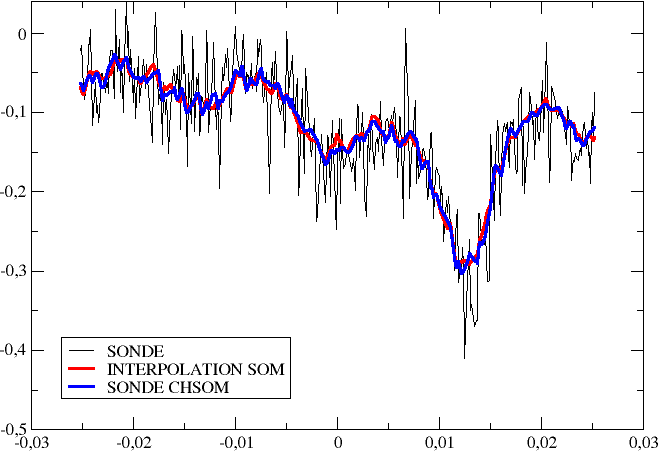
\includegraphics[width=\linewidth]{Figs/comparaison_sondes.png}
\end{minipage}
\begin{minipage}{0.5\linewidth}
\centering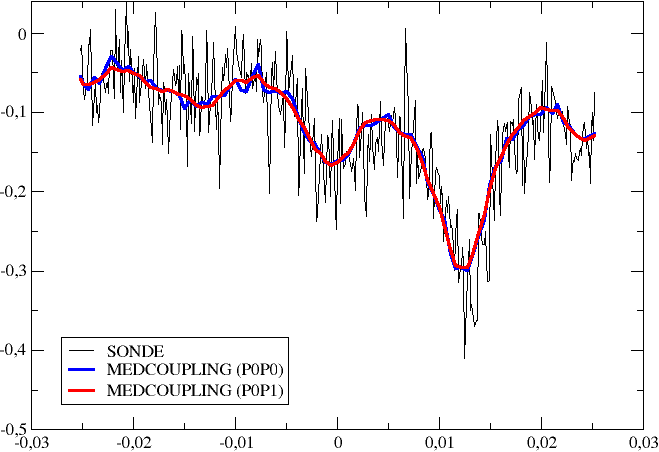
\includegraphics[width=\linewidth]{Figs/comparaison_medcoupling.png}
\end{minipage}
\caption{Diff\'erentes options de lissage d'un champ.}
\label{Fig=Interpolation}
\end{figure}

On propose donc d'\'ecrire par d\'efaut dans TrioCFD des champs d\'ej\`a liss\'es (par une m\'ethode \`a sp\'ecifier, la plus ad\'equate et la moins co\^uteuse en temps de
calcul) de fa\c con invisible pour l'utilisateur, tout en laissant la possibilit\'e \`a l'utilisateur expert de manipuler les interpolations. Cela permettrait une utilisation plus facile du code, notamment pour l'utilisateur d\'ebutant qui souhaite g\'en\'eralement obtenir une solution visuellement pr\'esentable sans n\'ecessairement se soucier des d\'etails d'interpolation des champs.

\begin{center}
\begin{longtable}{|l|l|} 
\hline
\rowcolor{couleur1}\multicolumn{2}{|c|}{Lot 1~: \'evolutions de l'existant}\\
\rowcolor{couleur2}\multicolumn{2}{|c|}{Sous-Lot 1.9~: Post-traitement}\\
%\rowcolor{couleur3}\multicolumn{2}{|c|}{T\^ache }\\
\hline Objectif &  \'ecrire par d\'efaut dans TrioCFD des champs d\'ej\`a liss\'es\\
& - conserver la possibilit\'e de manipuler les interpolations\\
\hline R\'ef\'erences & \`a d\'efinir  \\
\hline T\^aches \`a r\'ealiser &  impl\'ementation informatique et validation\\
\hline Conditionnement de l'action & Lot 1.8 achev\'e \\
\hline Risques identifi\'es &  ralentissement du code \\
\hline Charge de travail & R\&D court/moyen terme \\
\hline
\end{longtable}
\end{center}



% TURBULENCE TURBULENCE TURBULENCE TURBULENCE TURBULENCE TURBULENCE
% TURBULENCE TURBULENCE TURBULENCE TURBULENCE TURBULENCE TURBULENCE
\section{Mod\'elisation de la turbulence}
\label{section-turbulence}
\subsection{\'Etat des lieux}

Aujourd'hui, TrioCFD dispose d'un nombre limit\'e de mod\`eles de turbulence de type RANS, \`a savoir :

\begin{itemize}
	\item le mod\`ele $k$--$\varepsilon$ standard, avec loi de fermeture lin\'eaire du tenseur de Reynolds (l'approximation de Boussinesq) ;
	\item le mod\`ele $k$--$\varepsilon$ avec corrections bas Reynolds en proche paroi : plusieurs formulations ont \'et\'e impl\'ement\'ees en 2016 \cite{Peybernes2016} ;
	\item le mod\`ele $k$--$\varepsilon$ r\'ealisable, impl\'ement\'e en 2018 \cite{Angeli2018a} ;
	\item le mod\`ele $k$--$\varepsilon$ avec une loi de fermeture non lin\'eaire particuli\`ere (quadratique) du tenseur de Reynolds : le mod\`ele de Baglietto \cite{Baglietto2006}.
\end{itemize}


En RANS, les axes d'am\'elioration propos\'es concernent d'une part l'am\'elioration de certains mod\`eles existants, et d'autre part l'ajout de nouveaux mod\`eles. TrioCFD est peu performant sur la r\'esolution explicite de la totalit\'e de la couche limite, car il ne poss\`ede pas de mod\`ele pleinement op\'erationnel pour cela. 
Or il s'agit pourtant d'un besoin essentiel dans beaucoup d'applications, pour lesquelles on est actuellement limit\'e soit \`a l'utilisation de la loi de paroi standard avec l'inconv\'enient du domaine d'applicabilit\'e, soit au passage \`a la LES r\'esolue en paroi avec l'inconv\'enient du co\^ut de calcul. 

Des mod\`eles bas Reynolds ont \'et\'e impl\'ement\'es en 2016 pour am\'eliorer la situation, mais ils n'ont pas compl\`etement palli\'e le probl\`eme. On souhaite donc am\'eliorer les mod\`eles bas Reynolds existants, et en m\^eme temps ajouter les mod\`eles $k$--$\omega$ et $k$--$\omega$ SST, ces deux derniers \'etant d'autres mod\`eles de type bas Reynolds couramment employ\'es dans le monde industriel. On souligne de plus que l'utilisation de mod\`eles r\'esolvant finement la couche limite doit \^etre associ\'ee \`a la possibilit\'e de g\'erer les maillages hybrides prismes/t\'etra\`edres, afin de ne pas faire exploser le nombre de mailles dans la couche limite.

Il semble \'egalement int\'eressant d'impl\'ementer un mod\`ele de transport des tensions de Reynolds, dits RSM ({\og Reynolds Stress Model \fg}), afin d'am\'eliorer les simulations d'\'ecoulements dans les assemblages de r\'eacteurs nucl\'eaires.
En LES, les deux mod\`eles actuellement disponibles et op\'erationnels sont le mod\`ele de Smagorinsky standard et le mod\`ele WALE. On propose d'impl\'ementer dans le code \'egalement le mod\`ele de Smagorinsky dynamique.


\subsection{Mod\'elisation RANS de la turbulence}
\label{section-RANS}

\subsubsection{Am\'elioration des mod\`eles bas Reynolds et non lin\'eaires}
\label{Subsection=Bas_Reynolds}

Les mod\`eles bas Reynolds disponibles dans TrioCFD sont r\'ecapitul\'es dans le tableau~\ref{Tab=Mod\`eles_bas_Reynolds}. Le mod\`ele de Baglietto est un mod\`ele \`a fermeture non lin\'eaire, mais qui peut \^etre utilis\'e dans une version {\og haut Reynolds \fg} ou dans une version {\og bas Reynolds \fg}.

\begin{table}[!ht]
\begin{center}
\small
\begin{tabular}{|cccc|}
\hline
Mod\`ele	& Fermeture & Discr\'etisation & Thermique\\
\hline
Launder-Sharma & Lin\'eaire & VDF+VEF & Oui\\
Jones-Launder & Lin\'eaire & VDF+VEF & Oui\\
Lam-Bremhorst & Lin\'eaire & VEF & Oui\\
Baglietto & Non lin\'eaire & VEF & Oui\\
\hline
\end{tabular}
\end{center}
\caption{Mod\`eles bas Reynolds disponibles dans TrioCFD.}
\label{Tab=Mod\`eles_bas_Reynolds}
\end{table}

Un certain nombre de probl\`emes et difficult\'es li\'es \`a ces mod\`eles ont \'et\'e identifi\'es :

\begin{itemize}
	\item On observe assez souvent (presque syst\'ematiquement en VEF), que les grandeurs turbulentes ($k$, $\varepsilon$ ainsi que la viscosit\'e turbulente $\nu_t=C_\mu k^2/\varepsilon$) finissent par s'annuler. Quelques tests montrent que pour obtenir une solution turbulente non nulle, il faut que :

	\begin{enumerate}
		\item le nombre de Reynolds de l'\'ecoulement soit suffisamment \'elev\'e ;
		\item la viscosit\'e turbulente initiale soit suffisamment grande.
	\end{enumerate}

Ces conditions semblent \^etre n\'ecessaires et suffisantes en VDF, mais pas en VEF. En plus de la valeur initiale de $\nu_t$, les valeurs initiales de $k$ et $\varepsilon$, ainsi que la taille du maillage en proche paroi pourraient \'egalement avoir une influence sur ce ph\'enom\`ene. La figure~\ref{Fig=Bas_Reynolds} illustre la situation dans le cas d'un canal carr\'e. Les tests montr\'es ont \'et\'e men\'es avec le mod\`ele de Launder-Sharma mais les autres mod\`eles se comportent de mani\`ere similaire. En VDF, en partant d'une condition initiale telle que $\nu_t/\nu$ = 90, on obtient une solution turbulente pour un Reynolds de 6000, mais pas de 2000 ni de 4000. Il existe un seuil sur la valeur initiale de $\nu_t/\nu$ (ici entre 10 et 20 en VDF) en dessous duquel la turbulence finit par s'annuler compl\`etement. En VEF, il est presque impossible de capturer une solution turbulente non nulle, y compris avec des nombres de Reynolds \'elev\'es et une condition initiale \'elev\'ee. Cela rend l'utilisation de ces mod\`eles tr\`es difficile en VEF. Ces difficult\'es ont d\'ej\`a \'et\'e relev\'ees dans la note \cite{Peybernes2016}.\medskip
 	 
\begin{figure}[!ht]
\begin{minipage}{0.5\linewidth}
\centering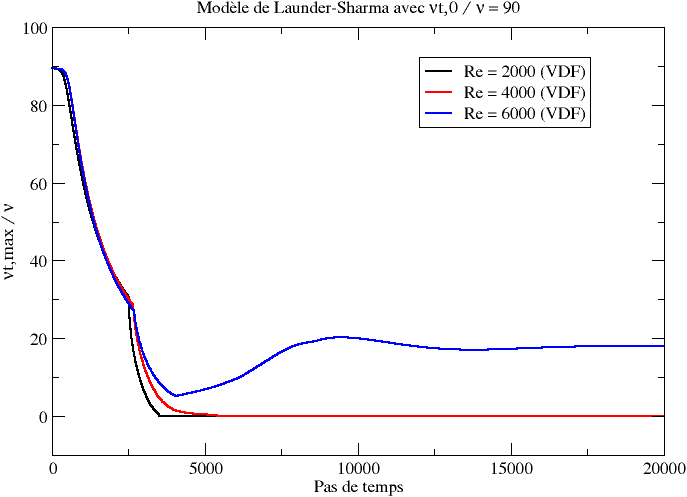
\includegraphics[width=\linewidth]{Figs/nut_max_Reynolds.png}
\end{minipage}
\begin{minipage}{0.5\linewidth}
\centering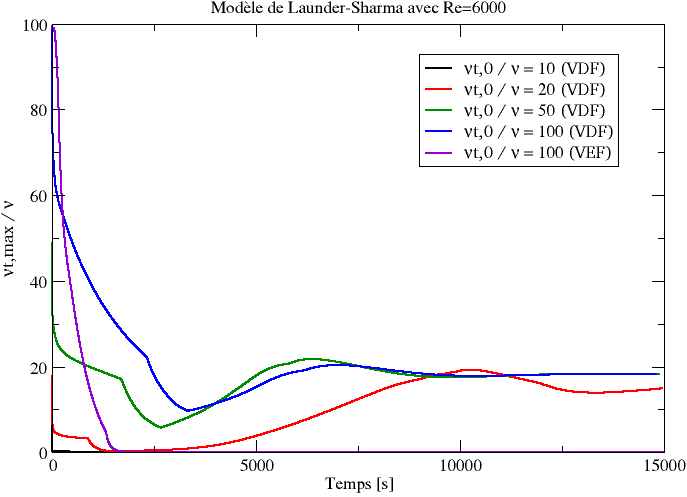
\includegraphics[width=\linewidth]{Figs/nut_max_VDF_VEF.png}
\end{minipage}
\caption{Illustration du comportement des mod\`eles bas Reynolds. \`a gauche : convergence de la viscosit\'e turbulente en fonction du nombre de Reynolds de l'\'ecoulement, en VDF. \`a droite : convergence de la viscosit\'e turbulente en fonction de sa valeur initiale, en VDF et VEF.}
\label{Fig=Bas_Reynolds}
\end{figure}

	\item L'utilisation de ces mod\`eles est parfois complexe notamment en raison des mots-cl\'es associ\'es susceptibles de provoquer des confusions. Le tableau~\ref{Tab=Mots_cl\'es_bas_Reynolds} r\'esume les mots-cl\'es dans chaque cas. On note que le mod\`ele de Lam-Bremhorst \cite{Lam1981} n\'ecessite un fichier suppl\'ementaire \`a g\'en\'erer s\'epar\'ement, de m\^eme que le mod\`ele de Baglietto utilis\'e dans sa version bas Reynolds.

\begin{table}[!ht]
\begin{center}
\small
\begin{tabular}{|c|l|}
\hline
Mod\`ele	& \multicolumn{1}{c|}{mots-cl\'es}\\
\hline
Launder-Sharma & \texttt{modele\_fonc\_bas\_Reynolds Launder\_Sharma \{ \}}\\
\hline
Jones-Launder & \texttt{modele\_fonc\_bas\_Reynolds\_Jones\_Launder \{ \}}\\
\hline
Lam-Bremhorst & \texttt{modele\_fonc\_bas\_Reynolds Lam\_Bremhorst \{}\\
& \texttt{fichier\_distance\_paroi ... \}}\\
\hline
Baglietto& \texttt{modele\_fonc\_bas\_Reynolds EASM\_Baglietto \{}\\
version {\og bas Reynolds \fg}) & \texttt{Reynolds\_stress\_isotrope 0 fichier\_distance\_paroi ... \}}\\
\hline
Baglietto & \texttt{modele\_fonc\_bas\_Reynolds standard\_keps \{}\\
(version {\og haut Reynolds \fg}) & \texttt{Reynolds\_stress\_isotrope 0 \}}\\
\hline
\end{tabular}
\end{center}
\caption{Mots-cl\'es associ\'es \`a chacun des mod\`eles.}
\label{Tab=Mots_cl\'es_bas_Reynolds}
\end{table}

L'activation de la relation de fermeture lin\'eaire ou non lin\'eaire du tenseur de Reynolds se fait avec le mot-cl\'e \texttt{Reynolds\_stress\_isotrope 0|1}, qui n'est cependant pas requis (le code ne renvoie pas d'erreur si ce mot-cl\'e n'est pas sp\'ecifi\'e) et dont l'effet n'est pas toujours \'evident pour l'utilisateur. Par exemple, dans les mots-cl\'es suivants : \texttt{Launder\_Sharma \{ Reynolds\_stress\_isotrope 0 \}}, il est difficile de savoir si l'on utilise le mod\`ele non lin\'eaire (donc de Baglietto) avec la correction bas Reynolds de Launder-Sharma, ou si \texttt{Reynolds\_stress\_isotrope 0} n'a pas d'effet. Autre exemple, est-ce que \texttt{standard\_keps \{ Reynolds\_stress\_isotrope 1 \}} signifie que l'on utilise le mod\`ele $k$--$\varepsilon$ standard ? De plus, il existe une confusion sur le mot-cl\'e \`a sp\'ecifier pour d\'efinir les conditions aux limites turbulentes aux parois : est-ce \texttt{paroi} ou \texttt{paroi\_fixe}, et quelle est la diff\'erence entre les deux ? Enfin, selon que le mod\`ele est {\og bas Reynolds \fg} ou non, il faut sp\'ecifier l'activation ou non de la loi de paroi, ce qui ajoute \`a la complexit\'e. Par exemple en bas Reynolds, il faut la d\'esactiver en utilisant le mot-cl\'e \texttt{turbulence\_paroi negligeable}.\medskip

	\item Des bugs ont \'et\'e report\'es dans le mod\`ele de Lam-Bremhorst, notamment dans les conditions aux limites.\medskip

	\item Ces mod\`eles sont tous utilisables en thermique mais cette partie n'a probablement pas \'et\'e compl\`etement valid\'ee.\medskip
\end{itemize}

On propose donc les r\'ealisations suivantes :\medskip

\begin{itemize}
	\item comprendre pourquoi les grandeurs turbulentes s'annulent (surtout en VEF) et trouver un moyen de rem\'edier \`a ce probl\`eme ;
	\item impl\'ementer les mod\`eles de Lam-Bremhorst et de Baglietto en VDF ;
	\item v\'erifier et corriger si n\'ecessaire le codage du mod\`ele de Lam-Bremhorst ;
	\item simplifier les mots-cl\'es appelant les mod\`eles bas Reynolds non lin\'eaires, supprimer les incoh\'erences et uniformiser les mots-cl\'es pour les conditions aux limites turbulentes ;
	\item valider ces mod\`eles en thermique.\medskip
\end{itemize}

Dans les mod\`eles \`a loi de fermeture non lin\'eaire, le tenseur de Reynolds s'\'ecrit comme une combinaison lin\'eaire de tenseurs \cite{Pope1975}. Ces tenseurs sont eux-m\^emes une somme de termes polynomiaux en S et R (respectivement le tenseur des taux de d\'eformation et le tenseur des taux de rotation), et sont d'ordre un \`a cinq. Ainsi, la valeur des coefficients de la combinaison d\'etermine si le mod\`ele est lin\'eaire (ordre un), quadratique (ordre deux), cubique (ordre trois), ... Dans la litt\'erature, il existe de nombreux mod\`eles non lin\'eaires qui diff\`erent essentiellement par la valeur de ces constantes. Par exemple, le mod\`ele de Baglietto impl\'ement\'e dans TrioCFD est un mod\`ele quadratique avec une modification des constantes initialement propos\'ees par Shih \textit{et al.} \cite{Shih1993}. Le mod\`ele de Craft \cite{Craft1996} est cubique. Pour g\'en\'eraliser l'impl\'ementation, on pourrait donc envisager de pouvoir rentrer manuellement dans le jeu de donn\'ees les constantes de la combinaison lin\'eaire.\\

\begin{center}
\begin{longtable}{|l|l|} 
\hline
\rowcolor{couleur1}\multicolumn{2}{|c|}{Lot 2: Mod\'elisation de la turbulence}\\
\hline
\rowcolor{couleur2}\multicolumn{2}{|c|}{Sous-Lot 2.1~: mod\`eles de type RANS.   }\\
\rowcolor{couleur3}\multicolumn{2}{|c|}{Tâche 2.1.a Mod\`eles bas Reynolds et non lin\'eaires}\\
\hline
T\^aches \`a r\'ealiser & - comprendre et solutionner le probl\`eme de l'annulation\\
& des grandeurs turbulentes\\
& - impl\'ementer les mod\`eles de Lam-Bremhorst et de\\
& Baglietto en VDF\\
& - v\'erifier (et corriger) le codage du mod\`ele de Lam-Bremhorst\\
& - simplifier et uniformiser les mots-cl\'es\\
& - valider ces mod\`eles en thermique\\
& - sp\'ecifier les constantes du mod\`ele non lin\'eaire\\
\hline

R\'ef\'erences & \cite{Shih1993,Craft1996,Baglietto2006,Pope1975,Lam1981,Peybernes2016}\\
\hline
Risques identifi\'es & Aucun \\
\hline
Charge de travail & Court terme: action en cours \\
\hline
\end{longtable}
\end{center}

\subsubsection{Mod\`eles $k$--$\omega$ et $k$--$\omega$ SST}

Bien que le mod\`ele $k$--$\varepsilon$ soit encore tr\`es populaire dans l'industrie, il poss\`ede de nombreux inconv\'enients connus. Parmi eux, il appara\^it que ce mod\`ele n'est pas bien pos\'e en tr\`es proche paroi : ainsi un raffinement croissant du maillage en proche paroi conduira \`a une erreur de mod\'elisation de plus en plus grande. On a alors le choix d'utiliser des lois de paroi (mais qui ne sont pas toujours valides), ou des corrections bas Reynolds (avec les difficult\'es mentionn\'ees en~\ref{Subsection=Bas_Reynolds}). On peut aussi changer de mod\`ele : le mod\`ele $k$--$\omega$ en particulier, dont la formulation de r\'ef\'erence a \'et\'e propos\'ee dans \cite{Wilcox1988}, ainsi que sa version {\og Shear-Stress Transport \fg} (SST) \cite{Menter1993}, sont g\'en\'eralement reconnus comme donnant de meilleurs r\'esultats que le $k$--$\varepsilon$ pour les \'ecoulements avec d\'ecollement de couche limite, et sont devenus \'egalement tr\`es populaires. Disposer de tels mod\`eles dans TrioCFD est devenu un r\'eel besoin pour nos applications \cite{Angeli2019a}.

Le mod\`ele $k$--$\omega$ est \'egalement un mod\`ele \`a deux \'equations : une \'equation de transport pour l'\'energie cin\'etique turbulente $k$, et une \'equation de transport pour le taux de dissipation turbulente sp\'ecifique $\omega$. Ce dernier se d\'efinit comme $\omega = \varepsilon/(k C_\mu)$, o\`u $C\mu = 0,09$ ($\omega^{-1}$ est donc une \'echelle de temps caract\'eristique de la turbulence). La viscosit\'e turbulente devient donc $\nu_t=k/\omega$. Ce mod\`ele peut \^etre utilis\'e avec une loi de paroi, mais a aussi l'avantage de pouvoir \^etre utilis\'e sur toute la couche limite sans correction suppl\'ementaire, et s'apparente dans ce cas \`a un mod\`ele bas Reynolds, car la grandeur $\omega$ se comporte asymptotiquement correctement \`a l'approche de la paroi (contrairement \`a $\varepsilon$). On n'a donc pas besoin de loi de paroi, mais d'un maillage suffisamment r\'esolu en proche paroi ($y^+ = 1$\footnote{y+=y*$u_\tau/\nu$ o\`u $y$ est la distance du premier point de maillage \`a la paroi, $\nu$ la viscosit\'e cin\'ematique et $u_\tau$ la vitesse de frottement ($u_\tau =\sqrt{\tau_p/\rho}$ avec $\tau_p$ la contrainte de cisaillement pari\'etale}). De plus, ce mod\`ele ne n\'ecessite pas le calcul des distances \`a la paroi, comme le mod\`ele de Lam-Bremhorst. Le mod\`ele $k$--$\omega$ est \'egalement plus performant que le mod\`ele $k$--$\varepsilon$ pour pr\'edire les interactions en proche paroi. Il a cependant quelques d\'efauts :\medskip

\begin{itemize}
	\item convergence plus difficile qu'avec le $k$--$\varepsilon$ ;
	\item sensibilit\'e plus grande aux conditions initiales et aux limites ;
	\item pr\'ecision inf\'erieure au $k$--$\varepsilon$ pour les \'ecoulements libres.\medskip
\end{itemize}

Le mod\`ele $k$--$\omega$ SST, propos\'e par Menter \cite{Menter1993}, est une association des deux mod\`eles de turbulence en fonction de la distance \`a la paroi : en proche paroi, il se comporte comme le mod\`ele $k$--$\omega$, et loin de la paroi comme le mod\`ele $k$--$\varepsilon$, avec un raccordement lisse par le biais de fonctions en tangente hyperbolique. Il n'a de sens que s'il est utilis\'e en tant que mod\`ele bas Reynolds : il combine alors les avantages de ces deux mod\`eles en \'eliminant leurs inconv\'enients.\medskip

On propose donc de r\'ealiser le travail suivant dans TrioCFD :\medskip

\begin{itemize}
	\item Compl\'eter l'impl\'ementation du mod\`ele $k$--$\omega$. Actuellement dans TrioCFD, il est disponible sous la forme d'un BALTIK, mais un travail de nettoyage des sources et de validation reste \`a r\'ealiser afin de le rendre vraiment fonctionnel.
	\item Impl\'ementer et valider le mod\`ele $k$--$\omega$ SST.
\end{itemize}


\begin{center}
\begin{longtable}{|l|l|} 
\hline
\rowcolor{couleur1}\multicolumn{2}{|c|}{Lot 2: Mod\'elisation de la turbulence}\\
\hline
\rowcolor{couleur2}\multicolumn{2}{|c|}{Sous-Lot 2.1~: mod\`eles de type RANS.   }\\
\rowcolor{couleur3}\multicolumn{2}{|c|}{T\^ache 2.1.b Mod\`eles $k$--$\omega$ et $k$--$\omega$ SST}\\
\hline
T\^aches \`a r\'ealiser & - compl\'eter l'impl\'ementation du mod\`ele $k$--$\omega$\\
& - impl\'ementer et valider le mod\`ele $k$--$\omega$ SST\\
\hline
R\'ef\'erences & \cite{Wilcox1988,Menter1993}\\
\hline
Risques identifi\'es & Aucun\\
\hline Conditionnement de l'action & Lot 2.1.a achev\'e \\
\hline
Charge de travail & Court terme \\
\hline
\end{longtable}
\end{center}

\subsubsection{Mod\`eles de tensions de Reynolds}

Le code TrioCFD monophasique ne dispose pas \`a l'heure actuelle de mod\`eles de tensions de Reynolds (RSM). Ces mod\`eles ne sont pas bas\'es sur une hypoth\`ese de viscosit\'e turbulente, mais sur des \'equations de transport des six composantes du tenseur de Reynolds. Ils permettent donc une repr\'esentation plus compl\`ete de la turbulence, au prix cependant d'un niveau de mod\'elisation \'elev\'e et d'un co\^ut de calcul important. Ils sont efficaces dans le cas d'\'ecoulements tournants (effet de {\og swirl \fg}), comme c'est le cas dans les assemblages de REP avec grilles de m\'elange, et pr\'esentent donc un int\'er\^et \'evident pour nos applications. L'impl\'ementation de tels mod\`eles doit \^etre envisag\'ee, mais n\'ecessite une phase bibliographique pr\'eliminaire et une \'evaluation plus approfondie des difficult\'es de mise en \oe{}uvre.


\begin{center}
\begin{longtable}{|l|l|} 
\rowcolor{couleur1}\multicolumn{2}{|c|}{Lot 2: Mod\'elisation de la turbulence}\\
\hline
\rowcolor{couleur2}\multicolumn{2}{|c|}{Sous-Lot 2.1~: mod\`eles de type RANS.   }\\
\rowcolor{couleur3}\multicolumn{2}{|c|}{T\^ache 2.1.c Mod\`eles de tensions de Reynolds (RSM)}\\
\hline
T\^aches \`a r\'ealiser &  - r\'ealiser une \'etude bibliographique sur les mod\`eles RSM\\
& - impl\'ementer et valider un mod\`ele RSM\\
\hline
R\'ef\'erences & \`A rechercher\\
\hline
Risques identifi\'es & Difficult\'es de mod\'elisation et de convergence\\
\hline Conditionnement de l'action & Lot 2.1.a achev\'e \\
\hline
Charge de travail & Long terme \\
\hline
\end{longtable}
\end{center}


\subsubsection{Production de turbulence li\'ee \`a la pouss\'ee d'Archim\`ede}

Le mod\`ele $(k,\epsilon)$ dit "r\'ealisable"~\cite{shih1995new, Shih1993, shih1995}, a \'et\'e d\'evelopp\'e dans TrioCFD courant 2018. 
Ce mod\`ele permet une meilleure \'evaluation de la viscosit\'e tourbillonnaire. Il repose sur les contraintes de positivit\'e de la composante normale des tensions de Reynolds et l'in\'egalit\'e de Schwartz pour les contraintes turbulentes transverses. Ce mod\`ele propose une nouvelle formulation de la viscosit\'e tourbillonnaire et une nouvelle \'equation du taux de dissipation, en se fondant sur l'\'equation dynamique des fluctuations de la vorticit\'e (et non de la vitesse, comme c'est le cas dans le mod\`ele k-epsilon standard). La nouvelle \'equation du taux de dissipation a l'avantage d'\^etre plus stable num\'eriquement et le mod\`ele r\'ealisable fournit de meilleurs r\'esultats sur de nombreux cas d'\'ecoulement, lorsque l'effet de la rotation sur les tensions de Reynolds est important. 


De la m\^eme mani\`ere que pour le mod\`ele $(k,\epsilon)$ dit \og r\'ealisable \fg, on souhaite pouvoir prendre en compte dans l'\'equation d'\'evolution du taux de dissipation turbulente 
$\varepsilon$ l'effet des variations de densit\'e li\'ees au caract\`ere anisotrope du fluide, que ce soit thermiquement ou dans sa composition, voire les deux \`a la fois. \\

\begin{center}
\begin{longtable}{|l|l|} 
\hline
\rowcolor{couleur1}\multicolumn{2}{|c|}{Lot 2~: mod\'elisation de la turbulence}\\
\rowcolor{couleur2}\multicolumn{2}{|c|}{Sous-Lot 2.1~: mod\`eles de type RANS.   }\\
\rowcolor{couleur3}\multicolumn{2}{|c|}{T\^ache 2.1.d~: Production de turbulence li\'ee \`a la pouss\'ee d'Archim\`ede: application au mod\`ele $(k,\epsilon)$ r\'ealisable}\\
\hline Objectif & - am\'eliorer la mod\'elisation RANS de la turbulence anisotrope   \\
\hline R\'ef\'erence & \cite{bahari, vanmaele}\\
\hline T\^aches \`a r\'ealiser &   - impl\'ementation  \\
& - validation  du mod\`ele  \\
\hline Charge de travail & R\&D moyen terme: action en cours \\
\hline
\end{longtable}
\end{center}

\subsubsection{Mod\'elisation RANS \`a partir de r\'eseaux de neurones}

Dans le domaine du calcul scientifique, les m\'ethodes actuelles utilisant l'apprentissage machine (Machine Learning) sont aujourd'hui examin\'ees pour mod\'eliser des
ph\'enom\`enes complexes. Plus particuli\`erement, le travail envisag\'e porte sur l'apprentissage d'un mod\`ele pour les tensions de Reynolds (g\'en\'eralisation de
l'hypoth\`ese de Boussinesq), et sur sa validation via son int\'egration dans TrioCFD. La mise en {\oe}uvre de la m\'ethodologie a d\'ebut\'e par le biais de deux stages
s'\'etant d\'eroul\'es conjointement avec le LGLS courant 2019 et ayant conduit \`a des r\'esultats tr\`es prometteurs. Nous avons utilis\'e des r\'eseaux de neurones
entra\^in\'es par apprentissage sur des calculs DNS de r\'ef\'erence, en utilisant l'architecture neuronale propos\'ee par Ling~\cite{ling2016reynolds}, qui permet notamment
de prendre en compte des contraintes de nature physique sur le tenseur de Reynolds (par exemple, l'invariance galil\'eenne). Les DNS de r\'ef\'erence men\'ees avec TrioCFD sont celles du canal \`a section carr\'ee et rectangulaire, qui sont des cas simples d'\'ecoulement monophasique, mais on souhaite \'elargir ces bases d'apprentissage. L'action future concerne la poursuite de la mise en {\oe}uvre de l'apprentissage machine (hyper-param\`etres, pr\'etraitements et post-traitements des donn\'ees) avec la biblioth\`eque TensorFlow, ainsi que la validation a posteriori des mod\`eles g\'en\'er\'es par le r\'eseau de neurones : il s'agira donc de les int\'egrer dans le code TrioCFD, puis de comparer les calculs RANS incluant ces mod\`eles avec les DNS de r\'ef\'erence.

\begin{center}
\begin{longtable}{|l|l|} 
\hline
\rowcolor{couleur1}\multicolumn{2}{|c|}{Lot 2~: mod\'elisation de la turbulence}\\
\rowcolor{couleur2}\multicolumn{2}{|c|}{Sous-Lot 2.1~: mod\`eles de type RANS.   }\\
\rowcolor{couleur3}\multicolumn{2}{|c|}{T\^ache 2.1.e~: Mod\'elisation RANS \`a partir de r\'eseaux de neurones}\\
\hline Objectif & apprentissage d'un mod\`ele pour les tensions de Reynolds  \\
\hline R\'ef\'erence & \cite{ling2016reynolds}\\
\hline T\^aches \`a r\'ealiser &   - impl\'ementation  \\
& - validation    \\
\hline Charge de travail & R\&D moyen terme: action en cours \\
\hline
\end{longtable}
\end{center}
 
\subsection{La simulation des grandes \'echelles}

L'id\'ee ma\^itresse est d'identifier, par r\'esolution directe, les caract\'eristiques de grande taille de l'\'ecoulement en ne mod\'elisant que des mouvements de petite taille. Une caract\'eristique tr\`es importante des m\'ethodes LES est que la r\'esolution spatiale d\'epend de la taille des mailles. Contrairement aux mod\`eles en un point, la variation de la taille des mailles aura, tout le temps, une influence sur les r\'esultats, m\^eme avec une discr\'etisation et une r\'esolution num\'erique id\'eale. A la taille de la maille correspond un filtrage spatial dont il faut d\'efinir les caract\'eristiques. Pour simuler les ph\'enom\`enes de taille inf\'erieure \`a celle de la maille, il faut utiliser un mod\`ele de sous-maille. 

Les mod\`eles de sous-mailles sont classiquement class\'es en deux cat\'egories~: les mod\`eles fonctionnels et les mod\`eles structurels.

\begin{itemize}
\item[-]
 Les mod\`eles fonctionnels reposent sur l'hypoth\`ese essentielle que l'interaction entre les \'echelles r\'esolues et les \'echelles mod\'elis\'ees est principalement de type \'energ\'etique. Ils cherchent ainsi \`a reproduire les transferts \'energ\'etiques entre les \'echelles r\'esolues et les \'echelles mod\'elis\'ees. 
L'exemple le plus connu est le mod\`ele de Smagorinsky. Le m\'ecanisme de transfert direct  d'\'energie est suppos\'e similaire \`a un m\'ecanisme de diffusion pilot\'e par une viscosit\'e artificielle ou viscosit\'e sous-maille, dont la formulation est donn\'ee par l'expression de Boussinesq. Ce mod\`ele est le plus couramment utilis\'e. Il est disponible dans TrioCFD.  Un deuxi\`eme mod\`ele fonctionnel ( mod\`ele de {\sc{Wale}}) est disponible.

\item[-]
Les mod\`eles structurels ont quant \`a eux pour but de reproduire le plus fid\`element possible les composantes des termes sous-maille. Leurs m\'ethodes de construction se  basent sur diff\'erents principes de d\'eveloppement math\'ematique. Par exemple, les mod\`eles de similarit\'e d'\'echelles sont construits sur diff\'erents niveaux de filtrage parmi les \'echelles r\'esolues. Plus r\'ecemment, des outils de math\'ematiques appliqu\'ees tels que les r\'eseaux de neurones commencent \`a \^etre utilis\'es. Aucun mod\`ele structurel n'a \'et\'e \'etudi\'e jusqu'\`a pr\'esent par les \'equipes de d\'eveloppement de TrioCFD. \\
\end{itemize}

\begin{rque}
Les m\'ethodes LES n\'ecessitent l'emploi de m\'ethodes num\'eriques tr\`es pr\'ecises, avec peu de viscosit\'e num\'erique et dissipation. 
\end{rque}

Plus sp\'ecifiquement \`a la composante VEF du code,  les deux mod\`eles de sous-maille suivants sont disponibles~: 
\begin{enumerate}
\item
le mod\`ele de {\sc{Smagorinsky}}, dans sa version de base~: il introduit une constante dont il faut ajuster la valeur \`a chaque configuration d'\'ecoulement. Il pr\'esente les autres limitations principales suivantes~:  il n'a pas le bon comportement au voisinage des parois (viscosit\'e turbulente non nulle), ne s'annule pas pour un \'ecoulement laminaire, et est trop dissipatif dans les r\'egions de transition laminaire/turbulent.
\item
le mod\`ele {\sc{Wale}}\footnote{Wall-adapting local eddy-viscosity model.}~\cite{WALE} pr\'esente des avantages par rapport au mod\`ele de Smagorinsky. En effet, sa viscosit\'e turbulente tend \`a s'annuler au voisinage de la paroi. Il produit une viscosit\'e turbulente nulle pour un \'ecoulement laminaire, et est invariant par translation et rotation du syst\`eme de coordonn\'ees.
\end{enumerate}

En LES, les mod\`eles actuellement impl\'ement\'es sont le mod\`ele de Smagorinsky standard \cite{Smagorinsky1963} et le mod\`ele WALE \cite{Nicoud1999}. Ces deux mod\`eles sont de nature statique : la viscosit\'e turbulente sous-maille est \'egale \`a une constante multipli\'ee par le carr\'e de la taille de maille et par une fonction de l'\'ecoulement moyen. L'id\'ee des mod\`eles dynamiques est d'adapter la {\og constante \fg} \`a la structure locale de l'\'ecoulement et \`a la g\'eom\'etrie, en la rendant variable en espace et en temps. Germano \cite{Germano1991} et Lilly \cite{Lilly1991} ont propos\'e des proc\'edures \`a cette fin, donnant naissance au mod\`ele de Smagorinsky dynamique. Ce mod\`ele conduit \`a des pr\'edictions plus physiques de l'\'ecoulement en palliant en partie les limitations bien connues du mod\`ele de Smagorinsky standard (mauvais comportement asymptotique de la viscosit\'e turbulente au voisinage des parois, pas d'annulation de la viscosit\'e turbulente pour un \'ecoulement laminaire, forte dissipation dans les r\'egions de transition laminaire/turbulent).

On propose les r\'ealisations suivantes~:
\begin{enumerate}
\item
Analyses comparatives des mod\`eles de {\sc{Smagorinsky}} et {\sc{Wale}} sur des configurations d'assemblages combustibles, des zones de d\'ecollement, avec des maillages quelconques.
\item
Mod\'elisation fonctionnelle~: impl\'ementation d'un mod\`ele de {\sc{Smagorinsky}} dynamique, selon la proc\'edure Germano-Lilly~\cite{Germano}. Il s'agit d'une adaptation du mod\`ele de Smagorinsky par un ajustement automatique de la constante en chaque point et \`a chaque pas de temps. Cela permet de mieux adapter le mod\`ele \`a la structure locale de l'\'ecoulement.
\item Mise en {\oe}uvre et \'etude comparative d'une m\'ethode r\'ecente de LES, dite "Entropy Viscosity Method", \cite{Guermond1,Guermondverif,Wang}, dans laquelle le coefficient de viscosit\'e turbulente est proportionnel au d\'efaut de bilan discret d'\'energie (obtenu en prenant le produit scalaire de l'\'equation de quantit\'e de mouvement discr\`ete par le champ de vitesse) localement en chaque maille.  C'est une m\'ethode qui dissipe moins d'\'energie que la m\'ethode de {\sc{Smagorinsky}} dans les zones bien r\'esolues, puisque dans celles-ci le bilan discret d'\'energie est quasiment nul.
\end{enumerate}
La r\'ealisation de simulations LES se heurte \`a une difficult\'e concernant la cr\'eation du maillage. En effet, celui ci doit v\'erifier certains crit\`eres qui
d\'ependent de la solution \`a calculer. Par exemple, la taille des mailles est fonction de l'\'echelle de Kolmogorov (plus petite \'echelle dissipative de l'\'ecoulement).
Dans le cadre d'\'etudes r\'ealistes pour lesquelles on ne conna\^it pas la solution a priori, il est n\'ecessaire de r\'ealiser une \'etude pr\'ealable (qui repose souvent sur des calculs RANS) pour construire le maillage adapt\'e \`a la LES.


\begin{center}
\begin{longtable}{|l|l|} 
\hline
\rowcolor{couleur1}\multicolumn{2}{|c|}{Lot 2~: mod\'elisation de la turbulence}\\
\rowcolor{couleur2}\multicolumn{2}{|c|}{Sous-Lot 2.2~: mod\`eles de sous-maille.   }\\
\rowcolor{couleur3}\multicolumn{2}{|c|}{T\^ache 2.2.a  Comparaison des mod\`eles  {\sc{Smagorinsky}}, {\sc{Wale}} et Entropy Viscosity Method}\\
\hline Objectif & - se r\'eapproprier et valider sur des maillages quelconques  les mod\`eles \\
& de sous-maille existants et les comparer \`a un nouveau mod\`ele \\
\hline R\'ef\'erence & \cite{Guermond1,Guermondverif,Wang} et autres \`a d\'efinir \\
\hline T\^aches \`a r\'ealiser & - Mise en {\oe}uvre du mod\`ele "Entropy Viscosity Method"; \\
& - simulations LES avec les trois mod\`eles {\sc{Smagorinsky}} et {\sc{Wale}} et Entropy Viscosity Method \\
& sur diff\'erentes configurations, int\'egrant des calculs de Turbulence Homog\`ene Isotrope;\\
&- d\'eveloppement des post-traitements n\'ecessaires pour calculer des spectres en espace~; \\
&- r\'evision des sources du code pour v\'erification de l'impl\'ementation informatique et \\
& des sch\'emas num\'eriques utilis\'es.\\
& - tests de Turbulence Homog\`ene Isotrope avec construction des spectres en espace ;\\
& - d\'efinition d'une base de tests pertinents pour les applications en lien avec \\
& les r\'eacteurs ; \\
\hline Charge de travail & R\&D moyen terme \\
\hline
\hline\rowcolor{couleur3}\multicolumn{2}{|c|}{T\^ache 2.2.b  M\'ethodologie de cr\'eation des maillages adapt\'es \`a la LES }\\
\hline Objectif & - d\'evelopper une m\'ethodologie pour construire les maillages adapt\'es aux \\
& contraintes de l'approche LES \\
\hline R\'ef\'erence & \`a d\'efinir  \\
\hline T\^aches \`a r\'ealiser 
&  R\'ealisation des fiches de validation\\
\hline Charge de travail & R\&D moyen terme \\
\hline
\hline\rowcolor{couleur3}\multicolumn{2}{|c|}{T\^ache 2.2.c  Mod\`ele de {\sc{Smagorinsky}} dynamique }\\
\hline Objectif & -am\'eliorer le mod\`ele de   {\sc{Smagorinsky}} \\
\hline R\'ef\'erence & \cite{Germano} et autres \`a d\'efinir \\
\hline T\^aches \`a r\'ealiser &   - impl\'ementation  du mod\`ele de   {\sc{Smagorinsky}} dynamique \\
\hline Charge de travail & R\&D moyen terme \\
\hline
\end{longtable}
\end{center}



% GD GD GD GD GD GD GD GD GD GD GD GD GD GD GD GD GD GD GD GD GD GD GD GD 
% GD GD GD GD GD GD GD GD GD GD GD GD GD GD GD GD GD GD GD GD GD GD GD GD

\section{Nouveaux sch\'emas de discr\'etisation spatiale}

\subsection{Sch\'emas d'ordre \'elev\'e pour les poly\`edres quelconques}
\label{section-GD}

\subsubsection{Introduction}
Pour la simulation de r\'egimes turbulents, il est souhaitable de se servir d'un sch\'ema d'ordre \'elev\'e afin de mieux capturer les tourbillons. De plus, pour le probl\`eme de Stokes, il a \'et\'e montr\'e dans \cite{GaLS19} que la mont\'ee en ordre permet de r\'eduire l'erreur de consistance, et ainsi de mieux satisfaire la contrainte de divergence nulle en r\'eduisant le nombre
de modes parasites pour la vitesse. Pour mod\'eliser plus finement les \'ecoulements en proche paroi, il faudrait \'egalement utiliser un maillage constitu\'e de prismes pr\`es de la paroi, et de t\'etra\`edres au centre de l'\'ecoulement. Ainsi, il serait judicieux de disposer d'un sch\'ema num\'erique d'ordre \'elev\'e, adapt\'e aux maillages polygonaux (poly\'edriques en $3D$). De nombreuses m\'ethodes de Galerkin discontinues sont disponibles pour impl\'ementer un tel sch\'ema \cite{Jame18b}.

Quels que soient les sch\'emas envisag\'es, les \'etapes d'\'evaluation sont les suivantes~:
%-------------%
\begin{itemize}
\item Impl\'ementer l'algorithme sur une maquette ind\'ependante du code TrioCFD.
\item Analyser l'int\'egration dans le code TrioCFD.
\item Industrialiser le sch\'ema selon son p\'erim\`etre d'utilisation.
\end{itemize}
%-----------%  
Afin de qualifier rigoureusement les nouveaux d\'eveloppements, il est n\'ecessaire de les tester de fa\c cçon pr\'ecise sur des cas acad\'emiques. Ainsi, il faudrait disposer dans la base logicielle TRUST d'un solveur r\'eellement stationnaire~; et de sch\'emas de r\'esolution de probl\`emes non lin\'eaires. Cela permettrait a minima de discerner les diff\'erentes sources d'erreurs. Il faut donc~:
%-------------%
\begin{itemize}
\item Disposer de solveurs lin\'eaires pour matrices de type $BA^{-1}B^T$, avec une matrice $A$ non n\'ecessairement diagonale.
\item Disposer de solveurs non lin\'eaires de type algorithmes de Newton.
\item Disposer d'une architecture de code souple, permettant d'autres sch\'emas que l'algorithme pr\'ediction-correction.
\end{itemize}
%-------------%
Le solveur PolyMAC~\cite{Gers18} propose un sch\'ema d'ordre $1$ adapt\'e aux maillages poly\'edriques. L'int\'egration de ce solveur \`a la plateforme TRUST est pr\'evue pour fin 2019. Le mod\`ele de donn\'ees de ce solveur pourra \^etre utilis\'e pour l'impl\'ementation d'une m\'ethode d'ordre \'elev\'e sur maillages poly\'edriques, ce qui n\'ecessitera une \'etape de formation \`a ce nouvel outil.

\subsubsection{Sch\'emas VEM et HHO}


Nous proposons une mont\'ee en comp\'etence progressive, en commen\c cant par coder les \'el\'ements finis de Taylor-Hood d'ordre $2$, tels que $(\velocity_h,p_h)\in\vec{P}_2\times P_1$, ce qui permettrait de disposer un solveur d'ordre $2$ de r\'ef\'erence pour les d\'eveloppements plus complexes~; et serait utile pour les travaux concernant les \'el\'ements finis multi\'echelle. En terme de nombre d'inconnues, ces \'el\'ements sont aussi co\^uteux que les \'el\'ements finis $\vec{P}_1^{NC}\times(P_0+P_1)$ cod\'es dans TrioCFD et fortement employ\'es par nos utilisateurs.

Puis nous pr\'evoyions d'impl\'ementer la m\'ethode de Galerkin discontinue SIPG pour des polyn\^omes d'ordre $1$ et $2$, tels que $(\velocity_h,p_h)\in\vec{P}_k^{disc}\times P_{k-1}^{disc}$, sur maillages de simplexes, avant de passer aux maillages g\'en\'eraux. Parall\`element, il est important d'\'etudier les m\'ethodes modernes VEM \cite{BBCM13} et HHO \cite{DiEL16} associ\'ees aux logiciels acad\'emiques Vem++ (F. Dassi, Milan) ou DisK++ \cite{CiDE18}. L'ouvrage \cite{CDGH17} fournit des r\'ef\'erences et indique des directions \`a suivre pour une impl\'ementation efficace. 

%------------%
\begin{center}
\begin{longtable}{|l|l|} 
\rowcolor{couleur1}\multicolumn{2}{|c|}{Lot 3~: Nouveaux sch\'emas de discr\'etisation spatiale}\\
\rowcolor{couleur2}\multicolumn{2}{|c|}{Sous-Lot 3.1~: Sch\'ema d'ordre \'elev\'e pour les poly\`edres quelconques}\\
\rowcolor{couleur3}\multicolumn{2}{|c|}{T\^ache 3.1.a  : Sch\'emas VEM et HHO}\\
\hline 
Objectif & Mont\'ee en ordre de pr\'ecision
\\
\hline
\'etapes & Bibliographie, tester les logiciels acad\'emiques.
       \\
       & Impl\'ementer une m\'ethode DG dans une maquette.
       \\
       & Organiser le code pour le calcul parall\`ele.
       \\
       & Stokes $2D$ puis $3D$ puis Osen puis Navier-Stokes.
       \\
       & Etudier l'int\'egration dans TrioCFD.
       \\
       & D\'ecider de l'industrialisation.
       \\
\hline 
R\'ef\'erences & M\'ethodes VEM \cite{BBCM13} et HHO \cite{DiEL16}
\\
\hline Risques & travail de recherche, complexit\'e de la mise en {\oe}uvre informatique dans un code existant\\
\hline Pr\'erequis & Architecture de code souple. \\
& R\'esolution de syst\`emes lin\'eaires par blocs. \\
& Parall\'elisme hybride. \\
& M\'ethode d'int\'egration num\'eriques sophistiqu\'ees (tesselation). \\
\hline Charge de travail & R\&D long terme.\\
\hline
\end{longtable}
\end{center}

\subsubsection{Autres sch\'emas}
%----------------------%
Dans ce paragraphe, on fait une liste bibliographique non-exhaustive de sch\'emas num\'eriques r\'ecents pour r\'esoudre le probl\`eme de Stokes sur lesquels il n'est pas pr\'evu de travailler  \`a ce stade sur la p\'eriode 2020-2025. Id\'ealement, il faudrait disposer d'une architecture de code suffisamment souple pour qualifier rapidement ces sch\'emas sur un certain nombre de cas-tests repr\'esentatifs.\\
\\
{\em A stable enriched Galerkin element for the Stokes problem} \cite{CGRT18}
\\
L'espace des vitesses de la discr\'etisation $\vec{P}_1-P_0$ est enrichi en ajoutant les fonctions $\vec{P}_0$ de sorte que $(\velocity_h,p_h)\in(\vec{P}_1+\vec{P}_0)\times P_0$. La formulation variationnelle est stabilis\'ee par une p\'enalisation des sauts de la partie $\vec{P}_0$ de la vitesse.\\
\\
{\em A finite element method by patch reconstruction for the Stokes problem using mixed formulation} \cite{LSYY19}.
\\
Les auteurs utilisent une m\'ethode des moindres carr\'es pour reconstruire une solution d'ordre \'elev\'e patch par patch, \`a partir d'une approximation $P_0$ sur les \'el\'ements. La m\'ethode s'applique \`a des maillages polygonaux.\\
\\
{\em A Divergence Free Weak Virtual Element Method for the
Stokes Problem on Polytopal Meshes} \cite{ChWa19}
\\
La pression est approch\'ee par des \'el\'ements finis discontinus et la vitesse est discr\'etis\'ee par des \'el\'ements finis virtuels conformes dans $\vec{H}(\mathrm{div})$. Cette m\'ethode permet de calculer une vitesse discr\`ete \`a divergence nulle. L'estimation d'erreur sur la vitesse est alors ind\'ependante de l'estimation d'erreur sur la pression. La m\'ethode est adapt\'ee \`a une discr\'etisation d'ordre \'el\'ev\'e sur maillages g\'en\'eraux.\\
\\
D'autres m\'ethodes plus anciennes pourraient pr\'esenter un int\'er\^et pour obtenir un sch\'ema num\'erique \'economique en terme d'empreinte m\'emoire~:
\\
\\
{\em A stable finite element for the Stokes equations} \cite{ArBF84}
\\
La vitesse est discr\'etis\'ee avec les \'el\'ements finis $\vec{P}_1$ enrichis par des bulles volumiques $\vec{P}_{BV}{}|_T=\{\prod_{i=1}^{d+1}\lambda_{i,T}\}^d$ et la pression est discr\'etis\'ee avec les \'el\'ements finis $P_1$, de sorte que $(\velocity_h,p_h)\in(\vec{P}_1+\vec{P}_{BV})\times P_1$. Ainsi, cette m\'ethode est \'econome en nombre d'inconnues. La conservation de la masse n'est pas locale, mais cela peut \^etre am\'elior\'e par des techniques de post-traitement, comme indiqu\'e dans \cite{JKMN17}. Ces \'el\'ements finis sont appel\'es les {\em mini-\'el\'ements}.\\
\\
{\em Analysis of some finite elements for the Stokes problem} \cite{BeRa85}
\\
La vitesse est discr\'etis\'ee avec les \'el\'ements finis $\vec{P}_1$ enrichis par des bulles surfaciques $\vec{P}_{BF}{}|_F=\{\prod_{i=1}^d\lambda_{i,F}\}^d$ et la pression est discr\'etis\'ee avec les \'el\'ements finis $P_1$, de sorte que $(\velocity_h,p_h)\in(\vec{P}_1+\vec{P}_{BF})\times P_1$. Cette m\'ethode est \'econome en nombre d'inconnues (plus que la m\'ethode pr\'ecit\'ee). La conservation de la masse n'est pas locale, mais cela peut \^etre am\'elior\'e par des techniques de post-traitement, comme indiqu\'e dans \cite{JKMN17}. Ces \'el\'ements finis sont appel\'es les {\em \'el\'ements finis de Bernardi-Raugel}. 
%--------------------------%
\subsubsection{Nombre d'inconnues} 
%--------------------------%
On donne le nombre approximatif d'inconnues en dimension $2$ et $3$ pour les sch\'emas sur simplexes, $N_T$ repr\'esentant le nombre de simplexes du maillage. Dans la derni\`ere colonne, on indique si on peut remplacer la matrice de masse de la vitesse par une matrice de masse diagonale.
\begin{table}[!h]
\begin{center}
\begin{tabular}{c|c|c|c|c}
El\'ements finis& $(\velocity_h,p_h)$ & $2D$ & $3D$ & $M_{diag}$\\
\hline
Stabilis\'es &$\vec{P}_1\times P_0$ stabilis\'es    & $2\,N_T$   & $1.5\,N_T$ &  oui \\
Bernardi-Raugel&$(\vec{P}_1+\vec{P}_{BF})\times P_1$& $3.5\,N_T$ & $4\,N_T$   &  ?   \\
Mini&$(\vec{P}_1+\vec{P}_{BV})\times P_1$& $3.5\,N_T$ & $4.3\,N_T$ &  ?   \\
Enrichis&$(\vec{P}_1+P_0)\times P_1$& $4\,N_T$   & $5\,N_T$   &  ?   \\
Crouzeix-Raviart&$\vec{P}_1^{NC}\times P_0$& $4\,N_T$   & $7\,N_T$   & oui  \\
Taylor-Hood&$\vec{P}_2\times P_1$& $4.5\,N_T$ & $7\,N_T$   & non  \\
TrioCFD&$\vec{P}_1^{NC}\times (P_1+P_0)$& $4.5\,N_T$ & $7.3\,N_T$ & oui
\end{tabular}
\caption{Nombre approximatif d'inconnues.}\label{tab:Ninc}
\end{center}
\end{table}




\subsection{Mod\'elisation pr\'ecise des milieux encombr\'es}
\label{section-poreux}
\subsubsection{Rappel de l'objectif~: calcul "CFD" d'une cuve compl\`ete de REP}
La simulation de l'\'ecoulement du fluide caloporteur dans l'ensemble du circuit primaire avec une approche CFD est aujourd'hui irr\'ealisable avec les moyens de calcul actuels. N\'eanmoins, on peut calculer pr\'ecis\'ement la solution du syst\`eme fluide en isolant un volume du circuit primaire, typiquement le pl\'enum inf\'erieur ou le pl\'enum sup\'erieur. La limite principale concerne le calcul de l'\'ecoulement dans le c{\oe}ur, compos\'e de nombreux assemblages, eux-m\^emes constitu\'es d'un grand nombre de crayons combustibles. 
L'objectif est de mettre en {\oe}uvre une mod\'elisation de la cuve compl\`ete avec la pr\'ecision la plus fine possible, \`a savoir une approche CFD pour le domaine complet, \`a l'exception du c{\oe}ur pour lequel on mettra en {\oe}uvre une nouvelle mod\'elisation ~\cite{FdR_Trio}.  

\`a ce jour, les m\'ethodes d\'evelopp\'ees  au STMF pour mod\'eliser la thermohydraulique du c{\oe}ur sont bas\'ees sur les \'equations d'Euler, compl\'et\'ees par une mod\'elisation homog\`ene des structures solides, c'est-\`a-dire par un mod\`ele poreux et des pertes de charges directionnelles : on mentionnera par exemple 

\begin{itemize}
\item
l'approche en maillage structur\'e d\'evelopp\'ee pour le c{\oe}ur d'ASTRID o\`u la section de passage axiale de chaque sous-canal d'un assemblage est trait\'ee avec six mailles et les effets des crayons sur l'\'ecoulement sont pris en compte par des corr\'elations empiriques issues d'exp\'eriences ;
\item
l'approche \`a l'\'echelle composant pour les c{\oe}urs de REP o\`u le maillage ne suit  ni la g\'eom\'etrie des sous-canaux ni celle des assemblages, qui permet de simuler l'\'ecoulement du fluide caloporteur \`a l'\'echelle de l'assemblage ou du sous-canal. M\^eme \`a l'\'echelle sous-canal, il est alors difficile de prendre en compte la complexit\'e des \'ecoulements transverses et le niveau de mod\'elisation reste tr\`es grossier.
\end{itemize}

L'objectif long terme est de d\'evelopper un mod\`ele c{\oe}ur beaucoup plus pr\'ecis que ceux mentionn\'es ci-dessus.

\subsubsection{Mise en {\oe}uvre d'une m\'ethode multi\'echelles}

Le travail a commenc\'e dans le cadre d'une th\`ese(~\cite{Feng2019}) consacr\'ee \`a la mise en {\oe}uvre d'une m\'ethode bas\'ee sur les \'el\'ements finis multi\'echelles~\cite{Allaire, Efendiev, Hou}. 

Dans cette approche, le nombre de degr\'es de libert\'e \`a calculer est comparable \`a celui issu des m\'ethodes d'homog\'en\'eisation, ce qui rend  les temps de calcul accessibles. Les informations locales (pr\'esence ou absence d'obstacles solides) sont prises en compte au travers des fonctions de base qui doivent \^etre calcul\'ees et qui contiennent, entre autres, les informations g\'eom\'etriques du milieu consid\'er\'e. Cette approche est
souvent appliqu\'ee pour les milieux poreux naturels en ing\'enierie p\'etroli\`ere. Le principe de la m\'ethode est, sur un maillage \`a l'\'echelle grossi\`ere, d'\'ecrire une formulation de Galerkin sur l'espace engendr\'e par les fonctions de base locales, celles-ci r\'esolvant un probl\`eme similaire avec des conditions aux limites particuli\`eres, sur un sous-maillage fin prenant en compte la g\'eom\'etrie pr\'ecise des obstacles.

Des travaux existent sur des milieux dits "perfor\'es"~\cite{Chung}, c'est-\`a-dire qui tiennent compte d'inclusions solides dans lesquelles l'\'ecoulement n'est pas consid\'er\'e. N\'eanmoins, \`a ce jour, peu de litt\'erature existe sur une application de type \'ecoulements dans les c{\oe}urs des r\'eacteurs qui peuvent s'apparenter \`a un "milieu perfor\'e". 

Des r\'esultats encourageants ont \'et\'e obtenus dans le cadre de la th\`ese de Q. Feng. Des gains de temps de calcul importants ont \'et\'e observ\'es avec des pertes de pr\'ecision limit\'ees \`a une dizaine de pourcents par rapport \`a des calculs DNS sur le maillage issu de la r\'eunion de tous les maillages fins des cellules grossi\`eres; par ailleurs, des calculs trop co\^uteux en DNS ont pu \^etre men\'es \`a bien avec cette approche. Un programme de travail pluriannuel, en collaboration avec le monde acad\'emique (G. Allaire), est en cours de d\'efinition pour poursuivre cette action. Quatre points principaux sont \`a d\'evelopper:
\begin{itemize}
\item L'enrichissement de l'espace des fonctions de base locales par des fonctions d'ordre plus \'elev\'e, et le calcul pr\'ecis de celles-ci, \'eventuellement par des m\'ethodes d'\'el\'ements finis d'ordre plus \'elev\'e \'egalement sur les maillages fins: analyse th\'eorique, impl\'ementation et estimation du gain effectif.
\item L'extension de la m\'ethodologie au calcul de cas-tests instationnaires.
\item La r\'ealisation d'un ensemble de cas-tests plus complets en trois dimensions d'espace; se pose en particulier une question d\'elicate d'intersection et d'abscence de tangence entre les cellules grossi\`eres et les obstacles, en sorte que les domaines ainsi obtenus restent connexes et facilement maillables.
\item  L'optimisation de l'ensemble de la cha\^ine de calculs dans le but d'industrialiser cette approche: g\'en\'eration du maillage grossier ; g\'en\'eration des sous-maillages fins prenant en compte les obstacles; calculs de fonctions de base sur ces maillages fins; assemblage et r\'esolution du probl\`eme sur le maillage grossier \`a l'aide des fonctions de base calcul\'ees; post-traitement de la solution ainsi obtenue.
\end{itemize}

\begin{center}
\begin{longtable}{|l|l|} 
\hline
\rowcolor{couleur1}\multicolumn{2}{|c|}{Lot 3~:Nouveaux sch\'emas de discr\'etisation spatiale}\\
\rowcolor{couleur2}\multicolumn{2}{|c|}{Sous-Lots 3.2~: Mod\'elisation fine des \'ecoulements en milieux encombr\'es}\\
\rowcolor{couleur3}\multicolumn{2}{|c|}{T\^ache 3.2.a~: \'el\'ements finis multi\'echelles}\\
\hline Objectif & D\'evelopper une mod\'elisation interm\'ediaire entre la CFD et la mod\'elisation \`a l'\'echelle \\
&composant\\
\hline R\'ef\'erences & \cite{jankowiak2018non,muljadi2015nonconforming,Feng2019} \\
\hline T\^aches \`a r\'ealiser & R\&D et travail de th\`ese \\
\hline Risques identifi\'es &  complexit\'e de la mise en {\oe}uvre informatique dans un code existant\\
\hline Charge de travail & R\&D long terme \\
\hline
\end{longtable}
\end{center}



\section{Maillage adaptatif, HPC et QI}
~\label{dd_qi}

\subsection{Estimateurs d'erreurs {\it{a posteriori}}}
\label{section-estimateurs-erreurs}

\subsubsection{Description de la m\'ethode}

Des progr\`es significatifs dans le domaine de la simulation en g\'en\'eral passeront par la quantification des incertitudes associ\'ees aux r\'esultats de simulation. Un
pr\'ealable (mais ce n'est pas le seul) \`a la ma\^itrise des incertitudes est la quantification de l'erreur entre la solution num\'erique et la solution exacte. L'estimation de cette erreur contribue \'egalement \`a la mise en {\oe}uvre de m\'ethodes adaptatives, qui permettent d'optimiser le rapport "pr\'ecision / co\^ut" en adaptant localement la finesse du maillage, ainsi que le pas de temps, en fonction des caract\'eristiques de la solution. 

Les th\'eories disponibles pour quantifier l'erreur sont tr\`es in\'egalement avanc\'ees selon les sch\'emas num\'eriques concern\'es. La discr\'etisation par \'el\'ements finis a l'avantage de mettre \`a disposition de nombreux outils th\'eoriques et pratiques pour obtenir des estimations d'erreurs {\it a priori} et {\it a posteriori}.

 Les estimations d'erreurs {\it a priori} permettent de d\'eterminer si la solution num\'erique issue d'une discr\'etisation converge vers la solution continue (qui en
 g\'en\'eral ne peut pas \^etre estim\'ee analytiquement), et surtout \`a quelle vitesse, ceci en fonction de la qualit\'e de l'approximation (typiquement du degr\'e des
 polyn\^omes pour une m\'ethode d'\'el\'ements finis) et de la r\'egularit\'e de la solution. Ces m\'ethodes permettent donc de d\'eterminer un ordre de convergence mais ne donnent pas acc\`es \`a l'erreur effective sur un maillage donn\'e. De telles estimations sont qualifi\'ees d'{\it a priori} car elles ne d\'ependent pas de la solution approch\'ee calcul\'ee.

A contrario, les estimations d'erreurs {\it a posteriori}, bas\'ees sur la solution discr\`ete obtenue, permettent de majorer l'erreur de discr\'etisation de fa\c con
explicite par des quantit\'es locales et calculables \`a partir de la solution discr\`ete approch\'ee calcul\'ee; ainsi il est possible d'adapter la discr\'etisation
(raffinement local du maillage, pas de temps adaptatif, \'eventuellement degr\'e des polyn\^omes) pour r\'eduire l'erreur globale. 
La th\'eorie des estimations {\it a posteriori} fait partie des outils math\'ematiques qui permettent de donner des indications sur une strat\'egie optimale d'am\'elioration des r\'esultats (au sens du meilleur rapport pr\'ecision / co\^ut du calcul) si la pr\'ecision recherch\'ee n'est pas atteinte par le calcul qui vient d'\^etre effectu\'e. 

Supposons par exemple que le mod\`ele continu revienne \`a r\'esoudre un syst\`eme d'\'equations, d'inconnues $U : M(U) = 0$ et que son approximation num\'erique revienne \`a r\'esoudre un syst\`eme approch\'e, d'inconnues $U_h : M_h(U_h) = 0$, la th\'eorie des estimations {\it a posteriori}, dont on peut faire remonter l'origine aux travaux de Babuska et Rheinboldt~\cite{Babuska1,Babuska2}, peut r\'epondre (au moins partiellement) aux souhaits formul\'es ci-dessus. En effet, ce type d'estimation est en g\'en\'eral une majoration de l'erreur du type $ \vert\vert  U - U_h\vert \vert \leq E(U_h, \mathcal T_h, f)$, o\`u $ E$ est une expression enti\`erement calculable qui d\'epend de la solution calcul\'ee $ U_h$  (mais jamais de la solution exacte $U$), du maillage $\mathcal T _h$ (maillage espace-temps pour les probl\`emes instationnaires), et des donn\'ees $f$ du probl\`eme (termes sources, conditions aux limites, conditions initiales, coefficients des \'equations...), toutes choses qui sont connues une fois le calcul effectu\'e (d'o\`u le nom d'estimations {\it a posteriori}). Plus encore, l'estimateur $E$ est en g\'en\'eral une somme de contributions locales (maille par maille) et, dans les travaux les plus r\'ecents, permettant de distinguer diff\'erentes sources d'erreurs (discr\'etisation spatiale, discr\'etisation temporelle, r\'esolution approch\'ee de syst\`emes non-lin\'eaires...), ce qui permet de savoir o\`u faire porter l'effort suppl\'ementaire (adaptation du maillage et/ou du pas de temps, meilleure r\'esolution du syst\`eme non-lin\'eaire...) en cas de pr\'ecision insuffisante du calcul. \\


\begin{rque}
Si l'on ne sait pas estimer correctement les erreurs num\'eriques dans un solveur d\'eterministe, il peut \^etre difficile, voire impossible d'interpr\'eter la propagation des incertitudes dans ce solveur, en raison de la d\'ependance de la pr\'ecision du solveur aux donn\'ees. Il est donc crucial de passer du temps \`a \'etablir ces estimations d'erreur, et de d\'eterminer comment elles influencent la propagation des incertitudes.  
\end{rque}

\subsubsection{Dans TrioCFD}

La R\&D propos\'ee ici sur les estimateurs d'erreurs concernera principalement  les estimateurs {\it a posteriori} et portera sur les sch\'emas num\'eriques d\'evelopp\'es dans TrioCFD.


\begin{center}
\begin{longtable}{|l|l|} 
\hline
\rowcolor{couleur1}\multicolumn{2}{|c|}{Lot 4~:Maillage adaptatif, HPC et QI }\\
\rowcolor{couleur2}\multicolumn{2}{|c|}{Sous-Lot 4.1~:estimations d'erreurs {\it a posteriori}}\\
\rowcolor{couleur3}\multicolumn{2}{|c|}{T\^ache 4.1.a:~analyses th\'eoriques }\\
\hline
Objectif & D\'evelopper une m\'ethode d'estimation d'erreur {\it a posteriori}  exploitable\\
& en vue de la mise en oeuvre d'une m\'ethode adaptative dans TrioCFD \\
\hline R\'ef\'erences &  \cite{Verfurth,Dari_duran_padra,carstensen_funken}\\
\hline T\^aches \`a r\'ealiser &  Obtenir un estimateur et l'adapter selon la discr\'etisation et le mod\`ele.\\
\hline Risques identifi\'es &  Les estimateurs d\'ependent des mod\`eles physiques et des m\'ethodes num\'eriques. \\
& En cas de changement de ceux-ci, les estimateurs doivent \^etre chang\'es.\\
\hline Charge de travail & R\&D moyen terme \\
\hline
\rowcolor{couleur3}\multicolumn{2}{|c|}{T\^ache 4.2.b~: mise en {\oe}uvre  }\\
\hline
Objectif & Mettre en {\oe}uvre un estimateur d'erreur {\it a posteriori}  \\
& en vue de simulations adaptatives dans TrioCFD \\
\hline R\'ef\'erences &   \\
\hline T\^aches \`a r\'ealiser & Impl\'ementation des diff\'erents termes des estimateurs  \\
\hline Risques identifi\'es &  Une fois que l'estimateur a d\'etermin\'e quelles zones du maillage sont \`a raffiner \\
& prioritairement, une phase de remaillage est n\'ecessaire si l'on souhaite am\'eliorer \\
& la qualit\'e de la solution, et un nouveau calcul doit \^etre ex\'ecut\'e \\
&  sur ce nouveau maillage. Un couplage it\'eratif  avec un logiciel de maillage\\
&   est donc n\'ecessaire. Dans le cas de probl\`emes instationnaires, \\
& des changements de maillage {\it en cours} de calcul sont n\'ecessaires, \\
& ce qui complique le processus. \\
\hline Conditionnement de l'action & Lot 4.2.b achev\'e \\
\hline Charge de travail & R\&D moyen terme \\
\hline
\end{longtable}
\end{center}


\begin{rque}
 
Cette action est engag\'ee par P. Omnes via le co-encadrement de la th\`ese de G. Nassreddine (d\'emarr\'ee en octobre 2017, financ\'ee int\'egralement par l'Universit\'e Paris 13), en co-direction avec Toni Sayah (Universit\'e Saint-Joseph de Beyrouth, Liban).
Il s'agit de prendre en compte deux sources d'erreur dans les estimations {\it a posteriori} pour Navier-Stokes incompressible: celle li\'ee \`a la discr\'etisation (spatiale et temporelle), et celle li\'ee \`a l'ajout du mod\`ele de turbulence, en deux dimensions puis en trois dimensions.
\end{rque} 
\begin{rque}
 
L'impl\'ementation d'un estimateur {\it a posteriori} pour les \'equations de Navier-Stokes stationnaires est pr\'evue en 2019; l'ajout du terme li\'e \`a la d\'ependance temporelle et de celui li\'e au mod\`ele de turbulence est pr\'evu pour 2020.
\end{rque} 



\subsection{D\'ecomposition de domaine}
\label{section-DD}
Un effort important portera sur l'impl\'ementation d'une m\'ethode de d\'ecomposition de domaine dans TrioCFD. L'objectif vis\'e est double: (i) l'am\'elioration des performances du code et (ii) la mise en {\oe}uvre d'une m\'ethode de parall\'elisme hybride adapt\'ee aux futures architectures des ordinateurs.

Apr\`es avoir rappel\'e les principes g\'en\'eraux des m\'ethodes de D\'ecomposition de Domaine (DD), on propose deux actions concernant~:

\begin{itemize}
\item[$-$]
la mise en {\oe}uvre d'une m\'ethode de DD en espace pour la r\'esolution de grands syst\`emes lin\'eaires, 

\item[$-$]
une m\'ethode de DD en espace-temps.
\end{itemize}

\subsubsection{Rappels sur les m\'ethodes de DD}
Les m\'ethodes de DD constituent un outil int\'eressant pour les simulations mettant en {\oe}uvre un grand nombre de degr\'es de libert\'e. Le principe g\'en\'eral est rappel\'e ici, \`a partir des r\'ef\'erences~\cite{Belliard} et~\cite{Ciobanu}.

On entend par DD la d\'ecomposition de l'espace vectoriel dans lequel on cherche la solution d'une \'equation aux d\'eriv\'ees partielles (EDP) en la somme d'espaces vectoriels de cardinal plus petit, dans lesquels la solution est plus facile \`a trouver. La solution de l'EDP initiale est donn\'ee par la composition de l'ensemble des solutions partielles. En d'autres termes, l'id\'ee de base consiste \`a s\'eparer un grand probl\`eme en petits sous-probl\`emes qui peuvent \^etre trait\'es en parall\`ele. C'est une forme de parall\'elisme. Ce formalisme permet

\begin{itemize}
\item[$-$]
de traiter des ph\'enom\`enes physiques de plus en plus compliqu\'es mod\'elis\'es par des EDP,
\item[$-$]
de traiter des probl\`emes de plus grande taille,
\item[$-$]
d'acc\'el\'erer la m\'ethode et d'obtenir une solution plus rapidement pour les simulations qui tournent d\'ej\`a hors formalisme DD.
\end{itemize}
L'efficacit\'e d'une m\'ethode de DD d\'epend directement de la m\'ethode utilis\'ee pour d\'ecomposer le domaine. Il existe un large spectre d'algorithmes de DD selon le type du probl\`eme \`a r\'esoudre (lin\'eaire, non-lin\'eaire, hyperbolique, elliptique,...). Diff\'erents niveaux de parall\'elismes peuvent \^etre consid\'er\'es. Nous en consid\'erons trois dans le pr\'esent plan de d\'eveloppement:

\begin{itemize}
\item[$-$]
le parall\'elisme en espace bas\'e sur la m\'ethode de Schwarz \`a chaque pas de temps,
\item[$-$]
le parall\'elisme en espace-temps connu sous le nom de relaxation d'ondes,
\item[$-$]
le parall\'elisme en temps, connu sous le nom d'algorithme parar\'eel.
\end{itemize}

\medskip

\begin{rque}
La m\'ethode de DD en espace-temps est d\'ej\`a en cours d'\'etude, avec une th\`ese qui a commenc\'ee en octobre 2016 et financ\'ee par le projet ANR CINEPARA. Des travaux pr\'eliminaires ont \'egalement \'et\'e r\'ealis\'es \`a l'occasion du CEMRACS 2016.
\end{rque}   

\subsubsection{DD en espace \`a chaque pas de temps}
Dans TrioCFD, on doit \`a chaque pas de temps r\'esoudre un probl\`eme en espace, dont la discr\'etisation m\`ene \`a des syst\`emes lin\'eaires de grande taille. On r\'esout ces derniers par des m\'ethodes it\'eratives (de type Gradient conjugu\'e, GMRES, ...).
La vitesse de convergence de ces m\'ethodes it\'eratives est li\'ee au conditionnement du syst\`eme lin\'eaire, qui se d\'egrade rapidement lorsque le pas du maillage devient petit; ceci a pour cons\'equence que le nombre d'it\'erations des solveurs it\'eratifs
augmente avec le nombre d'inconnues.

Le parall\'elisme actuel de TrioCFD est une forme de d\'ecomposition de domaine, au sens o\`u les t\^aches \`a faire pour calculer les diff\'erents \'el\'ements de la matrice finale sont r\'eparties sur diff\'erents processeurs. N\'eanmoins, in fine on r\'esout un syst\`eme ayant la taille du probl\`eme global. R\'epartir ainsi le travail des m\'ethodes it\'eratives en le partageant entre diff\'erents sous-domaines est certes utile mais ne r\'esout pas le probl\`eme du mauvais conditionnement et du nombre d'it\'erations n\'ecessaires \`a obtenir la convergence des m\'ethodes it\'eratives.
En outre, on peut montrer que les m\'ethodes de d\'ecomposition de domaine  de type Schwarz avec ou sans recouvrement des sous-domaines jouent un r\^ole de pr\'econditionneur
permettant de limiter l'augmentation (lorsque le pas du maillage d\'ecro\^it) du nombre d'it\'erations n\'ecessaires pour obtenir leur convergence. Ceci est d'autant plus vrai que l'on utilise des conditions de transmission d'ordre \'elev\'e, des coefficients optimis\'es \`a l'int\'erieur de celles-ci et une reformulation portant sur les seules inconnues d'interface. Un autre avantage est que les m\'ethodes de DD permettent d'augmenter la m\'emoire distribu\'ee disponible pour les simulations.

Cette action consiste \`a mettre en {\oe}uvre dans TrioCFD une m\'ethode de type Schwarz pour la r\'esolution d'une \'equation lin\'eaire de type elliptique typique de celle de TrioCFD (\'etape de projection pour le calcul de la pression). La validation de la m\'ethode reposera sur la r\'esolution de grands probl\`emes et une comparaison avec les performances obtenues par appel \`a la librairie {\sc{petsc}}.\\

\begin{rque}
Notons deux exemples de mises en {\oe}uvre d'une m\'ethode DD dans les codes "maison":

\begin{itemize}
\item le code de neutronique d\'eterministe du CEA (APOLLO3) poss\`ede son  propre solveur de syst\`emes lin\'eaires bas\'e sur une m\'ethode de Schwarz ;
\item comme mentionn\'e dans son m\'emoire de HDR, M. Belliard a d\'evelopp\'e une m\'ethode de DD  de type Schwarz pour la r\'esolution d'un probl\`eme elliptique (\'etape de projection du code GENEPI). Il a obtenu un gain significatif~\cite{Belliard}.
\end{itemize}
\end{rque}

\begin{center}
\begin{longtable}{|l|l|} 
\hline 
\rowcolor{couleur1}\multicolumn{2}{|c|}{Lot 4~: Maillage adaptatif, HPC et QI}\\
\rowcolor{couleur2}\multicolumn{2}{|c|}{Sous-Lot 4.2~: d\'ecomposition de domaine   }\\
\rowcolor{couleur3}\multicolumn{2}{|c|}{T\^aâche 4.2.a~:  m\'ethode de Schwarz pour la r\'esolution de syst\`emes lin\'eaires }\\
\hline Objectif & Disposer dans le code d'une m\'ethode pour la r\'esolution des syst\`emes \\
& lin\'eaires de grande taille, comme alternative aux solveurs \\
&de {\sc{petsc}} actuellement utilis\'es. \\
\hline R\'ef\'erences & \cite{Belliard} et autres \`a pr\'eciser \\
\hline T\^aches \`a r\'ealiser & - \'etude bibliographique ; \\
& - impl\'ementation informatique et validation~;\\
\hline Risques identifi\'es & La marge de progr\`es par rapport aux solveurs lin\'eaires de {\sc{petsc}}\\
& n'est pas \'evidente \`a pr\'evoir \\

\hline Charge de travail & R\&D moyen terme \\
\hline
\end{longtable}
\end{center}


\subsubsection{DD en espace-temps}
Pour des probl\`emes instationnaires, la dimension temporelle peut jouer un r\^ole important: au lieu de faire des it\'erations de Schwarz \`a tous les pas de temps, certaines m\'ethodes dites de relaxation d'ondes (OSWR pour "Optimized Schwarz Waveform Relaxation") permettent de ne faire des \'echanges entre processeurs qu'\`a la fin des it\'erations temporelles: au lieu de faire N (nombre de pas de temps) fois des communications de taille P (nombre d'inconnues d'interfaces), on fait une seule fois des communications de taille N*P, ce qui est nettement meilleur, \`a la fois parce qu'une seule synchronisation des processeurs est n\'ecessaire, mais aussi parce qu'il est plus rapide d'effectuer une fois des communications de taille N*P que N fois des communications de taille P. De telles m\'ethodes ont montr\'e leur int\'er\^et sur des probl\`emes d'\'ecoulements r\'egis par les \'equations de convection - diffusion~\cite{japhet2017space}.

\subsubsection{DD en temps}
Par ailleurs, lorsque le "budget processeurs" n'est pas encore compl\`etement d\'epens\'e par la parall\'elisation en espace (le nombre d'inconnues par processeur devenant
trop faible et les communications prenant de ce fait un temps excessif par rapport aux calculs eux-m\^emes), il existe des m\'ethodes de parall\'elisation en temps qui
permettent (sur certains probl\`emes en tout cas) de consommer de fa\c con plus optimale ce budget suppl\'ementaire: citons par exemple l'algorithme parar\'eel qui permet d'acc\'el\'erer les calculs en utilisant un syst\`eme pr\'edicteur (sur grille temporelle  -- et \'eventuellement spatiale -- grossi\`ere(s) et/ou avec un mod\`ele plus simple), calcul\'e s\'equentiellement (mais rapide d'ex\'ecution), puis correcteur calcul\'e en parall\`ele avec toute la pr\'ecision (temporelle, spatiale et de mod\`ele) souhait\'ee.

Un travail de R\&D "amont" est n\'ecessaire. Les difficult\'es \`a traiter sont d\'ecrites dans la section suivante.

\subsubsection{Travail th\'eorique}
\label{DD-temps-th\'eorie}
On peut distinguer quatre niveaux de difficult\'es:

\begin{itemize}
\item
on peut tout d'abord s'int\'eresser \`a l'approche la plus basique: Schwarz optimis\'e \`a chaque pas de temps  pour l'\'equation sur la vitesse $U*$, puis sur le Laplacien de pression \`a l'\'etape de projection. 
\item
OSWR pour Stokes et Navier-Stokes: ce travail a \'et\'e commenc\'e au CEMRACS pour Stokes puis dans la th\`ese de Duc Quang Bui: les coefficients optimaux pour les conditions de transmission de Robin ont \'et\'e obtenus en 2D d'espace; il faut g\'en\'eraliser au 3D et au non-lin\'eaire. Un aspect probablement tr\`es important est de savoir analyser ce qui se passe lorsque le Reynolds augmente.
\item
Utilisation de la m\'ethode parar\'eelle seule pour Navier-Stokes: il existe quelques exp\'eriences dans la litt\'erature~\cite{fischer2005parareal, steiner2015convergence}; il semble que des difficult\'es apparaissent \`a nombre de Reynolds \'elev\'e car le probl\`eme devient essentiellement convectif.
\item
Couplage avec le parar\'eel: il s'agit d'utiliser OSWR (avec peu d'it\'erations) comme solveur sur la grille temporelle fine et d'\'etudier quel est le meilleur compromis entre nombre d'it\'erations du parar\'eel et nombre d'it\'erations d'OSWR \`a l'int\'erieur des it\'erations de parar\'eel. Quelques publications traitent de ce probl\`eme dans d'autres contextes que celui de Navier-Stokes~\cite{hernandez2014quelques, gander2013parareal}. Des essais pour Stokes sont en cours dans le cadre de la th\`ese de D.Q. Bui.
\end{itemize}


\paragraph{Mise en {\oe}uvre informatique}
La mise en {\oe}uvre informatique des m\'ethodes ci-dessus cit\'ees sera tr\`es intrusive dans le code. Un bon moyen de proc\'eder pourrait \^etre de travailler d'abord dans une "maquette" pour isoler les choix les plus pertinents \footnote{ On pourra se rapprocher de M. Belliard qui a d\'evelopp\'e sa propre maquette pour ses travaux en lien avec GENEPI.} en s'affranchissant de la complexit\'e informatique. Ensuite, un travail d'impl\'ementation sera r\'ealis\'e dans le code, sachant que la difficult\'e identifi\'ee d\`es \`a pr\'esent est la suivante~: la DD est reformul\'ee comme un probl\`eme d'interface o\`u les inconnues sur lesquelles on it\`ere sont les seules inconnues aux interfaces entre les sous-domaines. Ainsi, au cours des it\'erations, on doit r\'esoudre des petits probl\`emes locaux dans chacun des sous-domaines, qu'il s'agit ensuite de post-traiter.

\begin{center}
\begin{longtable}{|l|l|} 
\hline
\rowcolor{couleur1}\multicolumn{2}{|c|}{Lot 4~: Maillage adaptatif, HPC et QI }\\
\rowcolor{couleur2}\multicolumn{2}{|c|}{Sous-Lot 4.2~:  d\'ecomposition de domaine  }\\
\hline\rowcolor{couleur3}\multicolumn{2}{|c|}{T\^ache 4.2.b. Travail th\'eorique d\'ecrit en section~\ref{DD-temps-th\'eorie}.}\\
\hline Objectif & Am\'eliorer les performances du code \\
\hline R\'ef\'erences &  \cite{japhet2017space, gander2013parareal, hernandez2014quelques, fischer2005parareal, steiner2015convergence} \\
\hline T\^aches \`a r\'ealiser &  analyse th\'eorique \\
\hline Risques identifi\'es &  travail de recherche\\
\hline Charge de travail & R\&D long terme \\
\hline
\rowcolor{couleur3}\multicolumn{2}{|c|}{T\^ache 4.2.c. Programmation.}\\
\hline Remarque &  T\^ache qui peut \^etre divis\'ee en plusieurs autres sous-t\^aches (\`a pr\'eciser ult\'erieurement) \\
\hline T\^aches \`a r\'ealiser &  - mise en {\oe}uvre informatique \\
\hline Risques identifi\'es &  travail de recherche\\
\hline Conditionnement de l'action & Lot 4.2.b achev\'e \\
\hline Charge de travail & R\&D long terme \\
\hline
\end{longtable}
\end{center}

\subsection{Analyse de sensibilit\'e}
\label{section-QI}
L'analyse de sensibilit\'e concerne la quantification des changements dans la solution d'un syst\`eme d'\'equations aux d\'eriv\'ees partielles (EDP) dus aux variations des
param\`etres d'entr\'ee du mod\`ele~\cite{chalons2018sensitivity, duvigneau2005evaluation,Shark_Fiorini,  hristova2006continuous, turgeon2001application}. 
Ce travail est le sujet du post-doctorat de C.Fiorini, commenc\'e le 15 octobre 2018, et qui consiste \`a appliquer l'analyse de sensibilit\'e aux probl\`emes de Navier-Stokes, en suivant deux axes, \`a savoir:  
\begin{itemize}
\item d\'erivation du syst\`eme d'\'equations par rapport aux param\`etres d'entr\'ee (par exemple conditions aux limites, propri\'et\'es physiques du fluide comme la viscosit\'e) par rapport auxquels il est souhaitable de r\'ealiser des \'etudes de sensibilit\'e
\item discr\'etisation des probl\`emes ainsi d\'eriv\'es et r\'esolution.
\end{itemize}

\subsubsection{\'etat d'avancement en 2019}

Dans un premier temps nous avons \'ecrit les \'equations de sensibilit\'e en utilisant la m\'ethode d'\'equation de sensibilit\'e continue. Nous avons \'etudi\'e la stabilit\'e du syst\`eme ainsi obtenu. 
Ensuite, le syst\`eme de sensibilit\'e a \'et\'e discr\'etis\'e selon la m\'ethode de type volumes \'el\'ements finis. La mise en {\oe}uvre de ce sch\'ema dans le code de
calcul TrioCFD a \'et\'e r\'ealis\'ee pour le cas o\`u le param\`etre d'int\'er\^et est  l'amplitude de la vitesse en entr\'ee.  La mise en {\oe}uvre dans le cas o\`u le param\`etre d'int\'er\^et est la viscosit\'e du fluide est en cours. 
Les objectifs \`a court terme sont d'analyser les r\'esultats des simulations et d'\'etablir l'influence des param\`etres sur la sortie du mod\`ele. Un article est en cours de r\'edaction. 
Dans un second temps,  une extension de ces travaux afin de consid\'erer le couplage avec la temp\'erature est pr\'evue.

\begin{center}
\begin{longtable}{|l|l|} 
\hline
\rowcolor{couleur1}\multicolumn{2}{|c|}{Lot 4~: Maillage adaptatif, HPC et QI}\\
\rowcolor{couleur2}\multicolumn{2}{|c|}{Sous-Lot 4.3~: Analyse de sensibilit\'e}\\
\hline\rowcolor{couleur3}\multicolumn{2}{|c|}{T\^ache 4.3.a.~: \'ecoulement laminaire}\\
\hline Objectif &  \'etablir l'influence des param\`etres sur la sortie du mod\`ele\\
\hline R\'ef\'erences &  ~\cite{chalons2018sensitivity, Shark_Fiorini,hristova2006continuous} \\
\hline T\^aches \`a r\'ealiser & - \'etude bibliographique ; \\
& - impl\'ementation informatique et validation~;\\
\hline Risques identifi\'es & aucun\\
\hline Charge de travail & R\&D court/moyen terme: action en cours \\
\hline
\end{longtable}
\end{center} 


\subsubsection{Objectifs pour 2020 }

Les objectifs principaux pour 2020 sont la finalisation de l'analyse et la mise en {\oe}uvre du couplage avec la temp\'erature, le passage en trois dimensions de l'espace et une deuxi\`eme publication. 

Enfin, un dernier objectif est la prise en compte de mod\`eles de turbulence. 

\begin{center}
\begin{longtable}{|l|l|} 
\hline
\rowcolor{couleur1}\multicolumn{2}{|c|}{Lot 4~: Maillage adaptatif, HPC et QI}\\
\rowcolor{couleur2}\multicolumn{2}{|c|}{Sous-Lot 4.3~: Analyse de sensibilit\'e}\\
\hline\rowcolor{couleur3}\multicolumn{2}{|c|}{T\^ache 4.3.b.~: Couplage avec la temp\'erature}\\
\hline Objectif & extension aux \'ecoulements thermohydrauliques \\
\hline R\'ef\'erences &  \`a pr\'eciser \\
\hline T\^aches \`a r\'ealiser & - \'etude bibliographique ; \\
& - impl\'ementation informatique et validation~;\\
\hline Risques identifi\'es & aucun\\
\hline Conditionnement de l'action & Lot 4.3.a achev\'e \\
\hline Charge de travail & R\&D court/moyen terme \\
\hline
\rowcolor{couleur3}\multicolumn{2}{|c|}{T\^ache 4.3.c.~: Prise en compte de la turbulence}\\
\hline Objectif &  extension aux \'ecoulements turbulents\\
\hline R\'ef\'erences &  \cite{turgeon2001application} et autres \`a pr\'eciser \\
\hline T\^aches \`a r\'ealiser & - \'etude bibliographique ; \\
& - impl\'ementation informatique et validation~;\\
\hline Risques identifi\'es & aucun\\
\hline Conditionnement de l'action & Lot 4.3.b achev\'e \\
\hline Charge de travail & R\&D moyen terme \\
\hline
\end{longtable}
\end{center}



\section{Nouvelles fonctionnalit\'es}
\label{section-nouvelles-fonctionalit\'es}
% ALE ALE ALE ALE ALE ALE ALE ALE ALE ALE ALE ALE ALE ALE ALE ALE ALE ALE ALE 
% ALE ALE ALE ALE ALE ALE ALE ALE ALE ALE ALE ALE ALE ALE ALE ALE ALE ALE ALE
\subsection{Mise en {\oe}uvre d'une m\'ethode ALE pour le couplage fluide-structure}
\label{section-ALE}


Il y a une attente forte concernant la mise \`a disposition dans TrioCFD d'une option ALE~\footnote{Il s'agit de prendre en compte dans la mod\'elisation fluide le d\'eplacement de la structure. Cela signifie que les n{\oe}uds du maillage n'ont pas une position fixe au cours du calcul.}  qui permettrait de simuler des probl\`emes d'interaction fluide-structure.  En effet, le projet ASSEMBLAGE a d'une part exprim\'e le besoin de disposer d'un code pour les calculs d'interaction fluide-structure pour \'etudier la d\'eformation des assemblages combustibles en cas de s\'eisme. D'autre part, le projet MECAN souhaiterait disposer d'une option ALE dans le code TrioCFD pour ses \'etudes sur les risques vibratoires des g\'en\'erateurs de vapeur. Les d\'eplacements solides \`a consid\'erer sont d'amplitudes vari\'ees. Par exemple, pour l'\'etude du risque vibratoire des g\'en\'erateurs de vapeur, on s'int\'eresse \`a des  d\'eplacements faibles \`a hautes fr\'equences. En outre, pour l'\'etude du d\'eplacement des assemblages combustibles en cas de s\'eisme, les structures solides sont susceptibles d'\^etre soumises \`a de grands d\'eplacements.



La strat\'egie de couplage fluide-solide retenue porte sur une approche partitionn\'ee. Le syst\`eme coupl\'e est r\'esolu \`a chaque pas de temps, sous-syst\`eme par sous-syst\`eme~\footnote{Le sous-syst\`eme en question est soit le domaine fluide soit le domaine solide.}, successivement ou it\'erativement. Des variables sont \'echang\'ees \`a l'interface fluide-solide. 
Nous avons fait le choix de cette approche en raison de sa flexibilit\'e : diff\'erents mod\`eles math\'ematiques, m\'ethodes num\'eriques et techniques
de discr\'etisation adapt\'es \`a chaque milieu (fluide et solide) peuvent \^etre utilis\'es s\'epar\'ement. 
Pour chaque milieu, un code de calcul sp\'ecifique est
utilis\'e, et la difficult\'e consiste \`a faire transiter l'information d'un code \`a l'autre afin de faire communiquer les deux milieux. 


Nous appelons le domaine commun $\Omega$, le domaine fluide $\Omega_F $ et le domaine solide $\Omega_S$.
Le couplage est r\'ealis\'e par des conditions aux limites \`a l'interface fluide-solide $\Gamma_{FS}$ reliant les vitesses et les contraintes dans le solide et le fluide. Les conditions suivantes sont impos\'ees sur $\Gamma_{FS}$:

\begin{equation}
  \left\{
\begin{array}{ll}
\velocity_F &= \velocity_S,\\
\vec{\sigma_F} \cdot \normal_F &= \vec{\sigma_S} \cdot \normal_S,
\end{array}
\right.
\label{cl_couplage}
\end{equation}

o\`u $\velocity_F$ et $\velocity_S$, $\vec{\sigma_F}$ et $\vec{\sigma_S}$, $\normal_F$ et $\normal_S$ sont respectivement la vitesse, le tenseur des contraintes et la normale ext\'erieure sortante  du fluide (variables indic\'ees par $F$) et du solide (variables indic\'ees par $S$).

Nous utilisons un formalisme classique dans lequel le fluide est trait\'e dans le r\'ef\'erentiel eul\'erien, tandis qu'un r\'ef\'erentiel lagrangien est consid\'er\'e pour le solide. Utilisant $(\ref{cl_couplage})$, les \'equations de Navier Stokes dans le r\'ef\'erentiel eul\'erien s'\'ecrivent:

\begin{equation}
  \left\{
\begin{array}{lll}
\ds{\frac{\partial \velocity}{\partial t} -\nabla. (\nu \vect{\nabla} \velocity) + \nabla. (\velocity  \otimes \velocity ) + \vect{\nabla}p }&=\vect{S},& \quad \text{dans}\quad \Omega_F, \\
\\
\ds{\nabla. \velocity }&= 0,& \quad \text{dans}\quad \Omega_F, \\
\\
\ds{\velocity }&= \velocity_d,& \quad \text{sur}\quad \Gamma_D \setminus \Gamma_{FS}, \\
\\
\ds{\velocity} &= \velocity_S,& \quad \text{sur}\quad  \Gamma_{FS}, \\
\\
\ds{(\nu \vect{\nabla} \velocity -p I_d)\cdot \normal  }&= \vec{ g},& \quad \text{sur}\quad \Gamma_N \setminus \Gamma_{FS},\\
\\
\ds{(\nu \vect{\nabla} \velocity -p I_d)\cdot \normal } &=  \vec{\sigma_S} \cdot \normal,& \quad \text{sur}\quad  \Gamma_{FS},
\end{array}
\right.
\label{eq:NS}
\end{equation}
o\`u $\partial \Omega = \Gamma_D \cup \Gamma_N \cup \Gamma_{FS}$, $\Gamma_D$ est la partie de fronti\`ere o\`u on applique les conditions de type Dirichlet et $\Gamma_N$ celle o\`u on applique les conditions de Neumann.

\subsubsection[Discr\'etisation spatiale]{Discr\'etisation spatiale du couplage fluide solide}

Afin de suivre l'interface fluide-solide, la m\'ethode Arbitraire Lagrange-Euler (ALE) est utilis\'ee.
Dans l'approche ALE, l'\'ecoulement fluide est calcul\'e sur un domaine qui est d\'eform\'e de fa\c con \`a suivre le mouvement de la fronti\`ere du solide. La vitesse de d\'eformation  ne suit  pas n\'ecessairement celle du fluide \`a l'int\'erieur du domaine.
On note $\vale$ cette vitesse du maillage fluide. Si $\vale$ est nulle, alors la m\'ethode se r\'eduit \`a une approche Eul\'erienne. Dans le cas  o\`u $\vale$ est \'egal \`a la vitesse du fluide nous retrouvons l'approche Lagrangienne. $\vale$ peut varier arbitrairement d'une valeur \`a l'autre dans le domaine fluide. Le calcul dans un tel domaine implique une reformulation des \'equations fluides dans ce rep\`ere.

Consid\'erons le r\'ef\'erentiel du laboratoire dans lequel les coordonn\'ees eul\'eriennes sont not\'ees $\vec{x}$ et les coordonn\'ees lagrangiennes li\'ees au solide sont not\'ees $\vec{X}$. 
Notons maintenant $\vec{\xi} $ les coordonn\'ees dans le maillage mobile de la formulation ALE. On peut les exprimer dans les coordonn\'ees lagrangiennes par $\vec{\xi} = \vec{\xi} (\vec{X},t)$ .

On d\'efinit alors le Jacobien $J$ et la vitesse du maillage mobile par:

$$ J (\vec{X},t) = \det \left(  \left.\frac{\partial \vec{\xi}}{\partial \vec{X}}\right|_{t} \right) (\vec{X},t),  $$

$$ \vale(\vec{X},t) =  \left.\frac{\partial \vec{\xi}}{\partial \vec{X}}\right|_{\vec{X}}  (\vec{X},t),$$

o\`u l'indice dans les d\'eriv\'ees partielles indique les variables qui restent constantes lors de la d\'erivation.


Soit $g$ une grandeur scalaire suffisamment r\'eguli\`ere, nous avons:

\begin{equation}
\left.\frac{\partial J  g}{ \partial t} \right|_{\vec{X}}  (\vec{X},t) =  J(\vec{X},t) \left( \left.\frac{\partial g}{ \partial t}\right|_{\vec{\xi}} +  \nabla_{\vec{\xi}}.(g \otimes \vale) \right) (\vec{\xi} (\vec{X},t), t ).
\label{transformation}
\end{equation}


En appliquant $(\ref{transformation})$ aux \'equations de Navier Stokes $(\ref{eq:NS})$ nous obtenons la formulation suivante:


\begin{equation}
\left\{
\begin{array}{ll}
\frac{\partial J \velocity}{\partial t} - J \left( \nabla_{\vec{x}}. (\nu \vect{\nabla} \velocity) \right)  + J \left( \nabla_{\vec{x}}. ( (\velocity - \vale) \otimes \velocity ) \right)  + J\vect{\nabla}p & =J\vect{S}, \\
\nabla_{\vec{x}}. ( \velocity - \vale )&=0.
\end{array}
\right.
\label{eq:NS_ALE}
\end{equation}

La m\'ethode ALE donne une formulation des \'equations de Navier-Stokes sous forme conservative avec une modification des vitesses de transport par la vitesse du maillage. 
Soit $g =  1$ dans  $(\ref{transformation})$, alors $J$ est solution de l'\'equation diff\'erentielle:
\begin{equation}
\left.\frac{\partial J}{\partial t}\right|_{\vec{X}}  (\vec{X},t) = J (\vec{X},t) \nabla_{\vec{\xi}}.(\vale)(\vec{\xi} (\vec{X},t), t ).
\label{jacobien}
\end{equation}

Le calcul de la vitesse du maillage doit v\'erifier  $(\ref{jacobien})$ mais doit aussi assurer que le maillage reste peu d\'eform\'e afin de garder des mailles non-retourn\'ees. Ceci peut \^etre assur\'e, par exemple en r\'esolvant l'\'equation:

\begin{equation}
\label{laplacien}
  \left\{
\begin{array}{ll}
\Delta \vale &= 0, \quad \text{dans}\quad \Omega_F, \\
\vale &= \velocity_S, \quad \text{sur}\quad \Gamma_{FS}, \\
\vale &= 0, \quad \text{sur} \quad \partial \Omega_F \setminus \Gamma_{FS}.
\end{array}
\right.
\end{equation}

D'autres m\'ethodes plus sophistiqu\'ees pourront \^etre test\'ees si besoin, voir par exemple~\cite{Bastinga}.

\subsubsection[Discr\'etisation temporelle]{Discr\'etisation temporelle du couplage fluide solide}
Les approches partitionn\'ees peuvent \^etre g\'en\'eralement divis\'ees en m\'ethodes faiblement coupl\'ees et fortement coupl\'ees. Dans les m\'ethodes faiblement coupl\'ees, un seul calcul
fluide et solide est effectu\'e \`a chaque pas de temps. Dans les m\'ethodes fortement coupl\'ees,
des sous-it\'erations sont utilis\'ees pour chacun des solveurs fluide et solide \`a chaque pas de temps.

Le couplage fluide solide bas\'e sur un algorithme partitionn\'e avec une discr\'etisation spatiale de type ALE peut \^etre  r\'esum\'e comme suit:

\begin{enumerate}
\item Le calcul de la vitesse du maillage $\vale$,
\item Proc\'edure de mise \`a jour du domaine fluide, 
\item Le calcul du Jacobien $J$,
\item R\'esolution des \'equations fluides dans le r\'ef\'erentiel ALE,
\item Traitement des conditions aux limites \`a l'interface fluide-solide,
\item Interpolation des donn\'ees lors du transfert d'un code  \`a l'autre (pour la prise en compte des conditions aux limites) car g\'en\'eralement les deux milieux (fluide et solide) ont des maillages  diff\'erents,
\item R\'esolution des \'equations solides dans le r\'ef\'erentiel lagrangien,
\item Transmission des grandeurs solide $\rightarrow$ liquide et liquide $\rightarrow$ solide suivant l'algorithme de couplage en temps choisi: explicite ou implicite.
\end{enumerate}



Dans un premier temps, on d\'eveloppera la m\'ethode pour des \'ecoulements laminaires ou des \'ecoulements turbulents pouvant \^etre calcul\'es avec une approche DNS (Lot
5.1.a). Dans un deuxi\`eme temps, il faudra prendre en compte la mod\'elisation de la turbulence, en commen\c cant par les mod\`eles de type RANS (Lot 5.2.c) puis en consid\'erant les mod\`eles de sous-maille pour la LES (Lot 5.2.d).

\begin{center}
\begin{longtable}{|l|l|} 
\hline
\rowcolor{couleur1}\multicolumn{2}{|c|}{Lot 5~: Nouvelles fonctionnalit\'es}\\
\rowcolor{couleur2}\multicolumn{2}{|c|}{Sous-Lot 5.1~:  m\'ethode ALE pour l'interaction fluide-structure}\\
\rowcolor{couleur3}\multicolumn{2}{|c|}{T\^ache 5.1.a~: domaine fluide, \'ecoulements laminaires}\\
\hline Objectif & prendre en compte l'effet du mouvement de la structure sur le fluide   \\
\hline R\'ef\'erences &  \cite{donea,  duarte, huvelin, souli} \\
\hline T\^aches \`a r\'ealiser &  -impl\'ementation informatique et validation pour~:\\
& - d\'eplacer les n{\oe}uds du maillage avec une vitesse impos\'ee et mettre \`a jour les\\
& quantit\'es g\'eom\'etriques ;\\
& - r\'esoudre les \'equations fluides dans le r\'ef\'erentiel mobile ;\\
\hline Charge de travail & Action r\'ealis\'ee \\
\hline
\rowcolor{couleur3}\multicolumn{2}{|c|}{T\^ache 5.1.b~: couplage du domaine fluide et du domaine solide }\\
%\rowcolor{couleur3}\multicolumn{2}{|c|}{T\^ache }\\
\hline Objectif &  mise en {\oe}uvre de l'algorithme de couplage fluide-structure ;   \\
\hline R\'ef\'erences & \cite{puscas, souli} et autres \`a d\'efinir \\
\hline T\^aches \`a r\'ealiser & - \'etude bibliographique pour d\'efinir la m\'ethode de couplage la mieux adapt\'ee aux\\
&  applications d'int\'er\^et ;\\
& - transmission des grandeurs solide $\longrightarrow$ liquide et liquide $\longrightarrow$ solide suivant \\
 &  l'algorithme de couplage en temps choisi ;\\
 \hline Charge de travail & R\&D court/moyen terme: action en cours  \\
\hline
\rowcolor{couleur3}\multicolumn{2}{|c|}{T\^ache 5.1.c~: domaine fluide, ALE avec mod\`eles RANS }\\
%\rowcolor{couleur3}\multicolumn{2}{|c|}{T\^ache }\\
\hline Objectif &  pouvoir r\'ealiser des calculs RANS sur maillages mobiles ; \\
\hline R\'ef\'erences &  \cite{koobus2000computation} et autres \`a d\'efinir\\
\hline T\^aches \`a r\'ealiser & - \'ecriture des \'equations RANS dans un r\'ef\'erentiel mobile et adaptation  \\
& du sch\'ema ;\\
& - impl\'ementation informatique et validation ;\\
 \hline Charge de travail & R\&D court/moyen terme: action en cours \\
\hline
\rowcolor{couleur3}\multicolumn{2}{|c|}{T\^ache 5.1.d~: domaine fluide, ALE avec mod\`eles LES }\\
%\rowcolor{couleur3}\multicolumn{2}{|c|}{T\^ache }\\
\hline Objectif &  pouvoir r\'ealiser des simulations LES sur maillages mobiles ;   \\
\hline R\'ef\'erences & \`a d\'efinir\\
\hline T\^aches \`a r\'ealiser & - adaptation des mod\`eles de sous-maille au cas d'un maillage mobile \\
& - impl\'ementation informatique et validation ;\\
\hline Conditionnement de l'action & Lot 5.1.c achev\'e \\
\hline
\end{longtable}
\end{center}



\begin{rque}
 
Les actions du lot 5.1.a ont \'et\'e r\'ealis\'ees en 2017, les d\'etails sont pr\'esent\'es dans le rapport technique~\cite{Steady_Adela_Reijo_2017}.  Les d\'eveloppements ont \'et\'e int\'egr\'es dans la version 1.7.9 de TrioCFD en juillet 2019. 
\end{rque}
\begin{rque}
Des actions concernant le lot 5.1.b ont eu lieu en 2018~\cite{NT_Reijo_Nikos} et 2019. 
Des actions visant la finalisation du lot 5.1.b et la r\'ealisation du lot 5.1.c sont en cours.   
\end{rque}



Par la suite, la r\'esolution de l'\'equation de l'\'energie dans le framework ALE doit \^etre mise en place. Afin de s'affranchir des difficult\'es li\'es \`a la mauvaise qualit\'e du maillage (qui impose un remaillage du domaine de calcul) suite \`a sa d\'eformation impos\'e par le d\'eplacement du solide, une technique plus efficace (plusieurs \`a disposition dans la litt\'erature) doit \^etre impl\'ementer. Ces techniques consistent principalement \`a remplacer le calcul de la vitesse du maillage via l'\'equation~\ref{laplacien} par des techniques plus sophistiqu\'ees mais beaucoup plus efficaces~\cite{wick2011fluid}. Enfin, l'\'evaluation des diff\'erents sch\'emas de couplage en temps est un point essentiel afin de garantir les propri\'et\'es de stabilit\'e et de consistance du sch\'ema de couplage. 


\begin{center}
\begin{longtable}{|l|l|} 
\hline
\rowcolor{couleur1}\multicolumn{2}{|c|}{Lot 5~: Nouvelles fonctionnalit\'es}\\
\rowcolor{couleur2}\multicolumn{2}{|c|}{Sous-Lot 5.1~:  m\'ethode ALE pour l'interaction fluide-structure}\\
\rowcolor{couleur3}\multicolumn{2}{|c|}{T\^ache 5.1.e~: \'equation de l'\'energie}\\
\hline Objectif & extension du domaine d'application \\
\hline R\'ef\'erences &  \`a d\'efinir \\
\hline T\^aches \`a r\'ealiser &  -impl\'ementation informatique et validation \\
& - r\'esoudre l'\'equation de l'\'energie dans le r\'ef\'erentiel mobile ;\\
\hline Conditionnement de l'action & Lot 5.1.c achev\'e \\
\hline Charge de travail & R\&D court/moyen terme \\
\hline
\rowcolor{couleur3}\multicolumn{2}{|c|}{T\^ache 5.1.f~: technique de d\'eformation du maillage }\\
%\rowcolor{couleur3}\multicolumn{2}{|c|}{T\^ache }\\
\hline Objectif &  am\'elioration de la  qualit\'e du maillage d\'eform\'e;   \\
\hline R\'ef\'erences & \cite{wick2011fluid} et autres \`a d\'efinir \\
\hline T\^aches \`a r\'ealiser & \'etude bibliographique, impl\'ementation et validation\\
\hline Conditionnement de l'action & Lot 5.1.b achev\'e \\
\hline Charge de travail & R\&D court/moyen terme\\
\hline
\rowcolor{couleur3}\multicolumn{2}{|c|}{T\^ache 5.1.g~: \'evaluation des diff\'erents sch\'emas de couplage en temps }\\
%\rowcolor{couleur3}\multicolumn{2}{|c|}{T\^ache }\\
\hline Objectif &  assurer des propri\'et\'es de stabilit\'e et consistance; \\
\hline R\'ef\'erences &  \`a d\'efinir\\
\hline T\^aches \`a r\'ealiser & - analyse, impl\'ementation informatique et validation ;\\
\hline Conditionnement de l'action & Lot 5.1.b achev\'e \\
\hline Charge de travail & R\&D court/moyen terme\\
\hline
\end{longtable}
\end{center}


\begin{rque}
Une th\`ese est propos\'ee en 2020 autour de ces actions d'interaction fluide-structure dans le framework ALE.  
\end{rque}


\subsection{Mod\'elisation polydisperse de particules solides}
\label{section-polydisperse}
Le code TrioCFD pourrait \^etre exploit\'e pour des \'etudes hydrodynamiques rattach\'ees \`a des proc\'ed\'es intervenant dans le cycle du combustible nucl\'eaire, plus
particuli\`erement au niveau de la mod\'elisation des proc\'ed\'es de pr\'ecipitation. Par le pass\'e, le code Trio\_U a \'et\'e  utilis\'e par le CEA de Grenoble et de
Cadarache pour la mise au point d'une mod\'elisation CFD pour d\'ecrire l'hydrodynamique d'un pr\'ecipitateur~\cite{HDR-MBertrand}. Un couplage avec la chimie avait \'et\'e
mis en place avec prise en compte des ph\'enom\`enes de microm\'elange pour simuler des \'ecoulements r\'eactifs par repr\'esentation de l'\'etat de s\'egr\'egation \`a
l'int\'erieur d'une maille de calcul.  La poursuite identifi\'ee \`a l'\'epoque de ces travaux concernait les d\'eveloppements polyphasiques permettant de prendre en compte
la pr\'esence de particules solides de tailles diff\'erentes au sein du pr\'ecipitateur.  L'objectif \'etait de pouvoir observer la distribution des cristaux form\'es au sein d'un r\'eacteur \`a effet vortex au cours d'une r\'eaction de pr\'ecipitation, en fonction de leur taille et de la vitesse d'agitation et d'identifier \'eventuellement des zones d'accumulation.

On propose ici d'impl\'ementer dans TrioCFD un mod\`ele Lagrangien de suivi de particules d'abord sous une forme monodisperse puis polydisperse. On s'inspirera des travaux de C. Morel concernant la proposition d'une mod\'elisation hydrodynamique appliqu\'ee au lit fluidis\'e~\cite{Morel}. 

\begin{center}
\begin{longtable}{|l|l|} 
\hline
\rowcolor{couleur1}\multicolumn{2}{|c|}{Lot 5~: nouvelles fonctionnalit\'es}\\
\rowcolor{couleur2}\multicolumn{2}{|c|}{Sous-Lot 5.2~:Mod\'elisation polydisperse de particules solides  }\\
\hline Objectif &   disposition d'une m\'ethode de suivi Lagrangien de particules solides \\
\hline R\'ef\'erences & \cite{HDR-MBertrand, Morel} \\
\hline T\^aches \`a r\'ealiser &  - compr\'ehension du besoin (g\'enie des proc\'ed\'es, CEA de Marcoule)  \\
& - analyse bibliographique, \\
& - impl\'ementation et validation.\\
\hline Risques identifi\'es & Ces d\'eveloppements ciblent les applications en lien avec les proc\'ed\'es de pr\'ecipitation. \\
& Bien identifier au pr\'ealable les \'equipes d\'esireuses d'exploiter TrioCFD.\\
\hline Charge de travail & R\&D court/moyen terme: en cours\\
\hline
\end{longtable}
\end{center}


\begin{rque}
Cette action a \'et\'e lanc\'ee dans le cadre du post-doctorat de Elie Saikali en 2019. Un rapport sera r\'edig\'e en 2020.
\end{rque}

\subsection{Mod\'elisation des \'ecoulements compressibles}
\label{section-compressible}
Afin d'\'elargir le champ d'applications du code, il pourrait \^etre int\'eressant de d\'evelopper un mod\`ele compressible. Cela permettrait par exemple de traiter certaines situations accidentelles avant \'ebullition et le passage \`a un mod\`ele diphasique envisag\'e dans le cadre de la strat\'egie pr\'esent\'ee dans le document~\cite{Metaphor}. 
D'autres applications envisageables seraient les simulations des \'ecoulements impliquant une large gamme de nombres de Mach, par exemple les \'ecoulements \`a la br\`eche et les applications de l'amont du cycle du combustible nucl\'eaire.

 
%Autres applications envisag\'ees sont les simulations des \'ecoulements impliquant une large vari\'et\'e de nombre de Mach. Des telles applications int\'eressent la DEN (par exemple les \'ecoulements dans les br\`eches) et la DAM (amont cycle).

  

\subsubsection{Sch\'ema de type Galerkin discontinu}

Dans l'\'eventualit\'e d'un tel d\'eveloppement,  un sch\'ema de type Galerkin discontinu pourra \^etre envisag\'e car :
\begin{enumerate}
\item
largement \'etudi\'e depuis une trentaine d'ann\'ees, il est relativement bien ma\^itris\'e aujourd'hui. C'est un argument fort en faveur d'une impl\'ementation dans un code industriel ;
\item
il est d'ordre de pr\'ecision quelconque, et de bonnes propri\'et\'es de stabilit\'e non lin\'eaire peuvent s'obtenir gr\^ace \`a une m\'ethode de stabilisation ;
\item
l'ordre de l'approximation polynomiale est d\'efini sur chaque \'el\'ement, c'est \`a dire localement. Il peut donc \^etre adapt\'e \`a l'\'ecoulement, en choisissant un ordre \'elev\'e dans les r\'egions de forte r\'egularit\'e de la solution, et un ordre faible au voisinage des discontinuit\'es (typiquement en pr\'esence de chocs);
\item
il permet de traiter des poly\`edres quelconques ;
\item
il est particuli\`erement adapt\'e au parall\'elisme.
\end{enumerate}

 L'impl\'ementation d'un tel sch\'ema sur base {\sc{trust}} sera assez rapide. L'effort le plus significatif portera sur la mise en place de la base de tests de validation.
 
 Les auteurs qui font  r\'ef\'erence pour les sch\'emas GD en compressible sont :
 \begin{itemize}
 \item
 Bassi et Rebay~\cite{Bassi-Rebay} ;
 \item
 Cockburn et Shu~\cite{Cockburn-Shu}, qui ont publi\'e ensemble sur le sujet et aussi s\'epar\'ement.
 \end{itemize}

On \'etudiera en particulier les variantes  Hybridizable Discontinuous Galerkin (HDG)~\cite{Cockburn-HDG}.

\begin{center}
\begin{longtable}{|l|l|} 
\hline
\rowcolor{couleur1}\multicolumn{2}{|c|}{Lot 5~: nouvelles fonctionnalit\'es}\\
\rowcolor{couleur2}\multicolumn{2}{|c|}{Sous-Lot 5.3~: \'ecoulements compressibles }\\
\rowcolor{couleur3}\multicolumn{2}{|c|}{T\^ache 5.3.a~: sch\'ema GD}\\
\hline Objectif &simulation des \'ecoulements compressibles  \\
\hline R\'ef\'erences & \cite{Cockburn-HDG} et autres \`a pr\'eciser   \\
\hline T\^aches \`a r\'ealiser &  - analyse des m\'ethodes HDG ;\\
& - impl\'ementation informatique \\
& - construction d'une base de validation pour les \'ecoulements compressibles.\\
\hline Risques identifi\'es & - ressources disponibles ayant peu d'exp\'erience sur les probl\`emes hyperboliques  \\
\hline Charge de travail & R\&D moyen terme\\
\hline
\end{longtable}
\end{center}

\begin{rque}
A ce jour, aucune action n'est engag\'ee sur ce lot.
\end{rque}

\subsubsection{Sch\'ema implicite de type Rosenbrock}

L'approximation d'\'ecoulements impliquant une grande h\'et\'erog\'en\'eit\'e du nombre de Mach est un challenge pour la simulation num\'erique. Depuis que Klainerman et Majda~\cite{klainerman1981singular,klainerman1982compressible} ont formul\'e math\'ematiquement la transition des \'equations de Navier-Stokes compressible \`a incompressible, un nombre consid\'erable de travaux ont \'et\'e d\'edi\'es \`a la production de sch\'emas num\'eriques capables de capturer efficacement tous les r\'egimes de compressibilit\'e. 
Malgr\'e des progr\`es notables dans ce domaine, des difficult\'es subsistent qui justifient de nombreuses publications r\'ecentes (par exemple~\cite{chalons2016all,dellacherie2016construction,fuster2018all,moguen2015godunov}). 

Ce th\`eme de recherche int\'eresse particuli\`erement le Commissariat \`a l'\'energie Atomique (CEA), tant \`a la Direction de l'\'energie Nucl\'eaire (DEN)~\cite{chalons2016all,cordier2012asymptotic,dellacherie2016construction} qu'\`a la Direction des Applications Militaires (DAM)~\cite{labourasse2019low,moguen2015godunov}, confront\'e \`a des applications impliquant des transitions violentes de r\'egimes. Un exemple pour les applications de la DEN est la rupture de conduite ou de cuve d'un R\'eacteur \`a Eau Pressuris\'ee (REP). 

Un post-doctorat commun DEN/DAM est envisag\'e prochainement. L'objectif de ce post-doctorat est de concevoir une souche de sch\'emas conservatifs et robustes permettant de simuler des \'ecoulements dans tous les r\'egimes de compressibilit\'e. Pour cela, le candidat retenu b\'en\'eficiera de l'expertise du CEA DAM en hydrodynamique compressible, et de celle du CEA DEN dans le r\'egime incompressible. 

Apr\`es une premi\`ere phase d'analyse num\'erique, il implantera, en 1D/2D, le sch\'ema choisi dans la plateforme JERICHO, dans laquelle sont d\'ej\`a impl\'ement\'es de nombreux sch\'emas pour le compressible. Ce sch\'ema sera ensuite test\'e sur des cas-tests acad\'emiques repr\'esentatifs des probl\`emes types \`a l'aide des moyens de calcul mis \`a disposition (TGCC). Le candidat s'inspirera du solveur de Poisson de TrioCFD pour la r\'esolution du syst\`eme lin\'eaire. Apr\`es avoir converg\'e sur une m\'ethode efficace, celle-ci sera report\'ee dans TrioCFD. Cela permettra une validation code \`a code.

R\'esultats attendus : 
\begin{itemize}
\item m\'ethodes num\'eriques conservatives et robustes, capables de traiter les \'ecoulements \`a tout nombre de Mach adapt\'ees au contexte HPC
\item extension incompressible de JERICHO et compressible de TrioCFD
\item communications et publications de niveau international.
\end{itemize}

\begin{center}
\begin{longtable}{|l|l|} 
\hline
\rowcolor{couleur1}\multicolumn{2}{|c|}{Lot 5~: Nouvelles fonctionnalit\'es}\\
\rowcolor{couleur2}\multicolumn{2}{|c|}{Sous-Lot 5.3~: \'ecoulements compressibles }\\
\rowcolor{couleur3}\multicolumn{2}{|c|}{T\^ache 5.3.b~: sch\'ema Rosenbrock}\\
\hline Objectif &simulation des \'ecoulements compressibles  \\
\hline R\'ef\'erences & \cite{chalons2016all,dellacherie2016construction,fuster2018all,moguen2015godunov} et autres \`a pr\'eciser   \\
\hline T\^aches \`a r\'ealiser &  - analyse de la m\'ethode Rosenbrock ;\\
& - impl\'ementation informatique \\
& - construction d'une base de validation pour les \'ecoulements compressibles.\\
\hline Risques identifi\'es & - ressources disponibles ayant peu d'exp\'erience sur les probl\`emes hyperboliques  \\
\hline Charge de travail & R\&D moyen terme\\
\hline
\end{longtable}
\end{center}

\subsection{Couplage avec la chimie via SCORPIO}
\label{section-scorpio}

Certaines applications n\'ecessitent la r\'esolution d'un syst\`eme de transport r\'eactif complet, telles que le colmatage des g\'en\'erateurs de vapeur, 
les couplages entre turbulence et \'echange chimique dans les r\'eacteurs agit\'es ou le stockage souterrain de d\'echets nucl\'eaires ou de CO$_2$. Dans un premier temps, on souhaite 
s'attaquer \`a la r\'esolution d'un syst\`eme de transport r\'eactif en milieu aqueux, avec pr\'esence \'eventuelle d'une phase solide, dans le contexte de mod\'elisation suivant:  

\begin{itemize}
\item \'ecoulement monophasique
\item transport : convection et diffusion-dispersion
\item chimie aqueuse
\item r\'eactions \`a l'\'equilibre ou sous cin\'etique
\item si phase solide:
\begin{itemize}
\item milieu poreux non-d\'eformable \`a porosit\'e variable $\omega$
\item chimie interphasique : pr\'ecipitation-dissolution, sorption
\item chimie solide : solutions solides, corrosion
\end{itemize}
\end{itemize}

On peut \'ecrire un tel syst\`eme sous la forme g\'en\'erale suivante: 

$$
\left\{
\begin{array}{lclr}
\partial _t(\omega a_k)  & = &  \displaystyle -div(a_k
 \vec{U} - \stackrel{\Rightarrow}{D}_k 
 (\vec{U}) \vec{\nabla} a_k ) + {\cal R}_k &
 \forall i \in [1,N_a]\\
\partial _t(\omega f_j)  & = & {\cal R}_j &
 \forall j \in [1,N_f]\\
\omega  & = & \displaystyle \omega ^0
\frac{1+f_{mv}^0}{1+f_{mv}} & \mbox{ avec }  f_{mv} = \sum _j {\cal V}_j^{mol} f_j \\
{\cal R}_{k/j} & = & \displaystyle \frac{1}{V_T} \sum _{r=1}^{N_r}
{\nu}_{k/j}^r I_r &
 \forall i \in [1,N_a]
 \forall j \in [1,N_f] \\
{\cal E}_{r} ( a_k , F_j ) & = & 0 & \forall r \in \mbox{ \'equilibres } \\
I_r & = & {\cal K}_{r} ( a_k , F_j  ) & \forall r \in \mbox{ cin\'etiques }
\end{array}
\right.
$$

Les param\`etres de transport et la temp\'erature seront d\'eduits d'une simulation thermohydraulique r\'ealis\'ee par TrioCFD.  
On observe que ce syst\`eme associe des ph\'enom\`enes de transport qui sont {\bf globaux et lin\'eaires} \`a des transferts chimiques qui sont \`a l'inverse {\bf locaux et non-lin\'eaires}. La r\'esolution num\'erique de ce genre de syst\`eme pose un certain nombre de probl\`emes: 

\begin{itemize}
\item fonction chimiques non-lin\'eaires (lois d'action de masse ou cin\'etiques) 
\item raideur en temps due aux effets thermiques ou aux catalyseurs
\item variables locales en nombre \'elev\'e (concentrations...)
\item contraintes de positivit\'e sur les concentrations (alors que des solutions existent dans l'espace des concentrations n\'egatives)
\end{itemize}

Une strat\'egie classique dans le milieu industriel consiste \`a proc\'eder par une approche s\'equentielle, ou d\'ecoupl\'ee, \'eventuellement it\'erative (SIA: Sequential Iterative Approach). 
Selon cette approche, d\'ecrite plus en d\'etail dans l'annexe \ref{section-decouplage}, on r\'esout s\'epar\'ement le transport par un unique syst\`eme global mais lin\'eaire et la chimie par 
autant de petits syst\`emes locaux non-lin\'eaires qu'on a choisi de Volumes \'el\'ementaires Repr\'esentatifs (VER), du point de vue chimique. Ces VER peuvent \^etre identiques aux 
cellules du maillage ou correspondre \`a un maillage plus grossier, superpos\'e au maillage utilis\'e pour le transport et/ou la thermohydraulique. 

Dans ce contexte, on propose de coupler TrioCFD avec un code con\c cu sp\'ecifiquement pour la r\'esolution de syst\`emes de transport r\'eactif: SCORPIO. 
 SCORPIO est un prototype d\'evelopp\'e au LMSF, associ\'e \`a SIDES, un solveur non-lin\'eaire comportant des int\'egrateurs temporels complexes et des m\'ethodes permettant d'\'eviter les solutions \`a concentrations n\'egatives, est utilis\'e notamment dans le code PAREX+. De plus, SCORPIO et SIDES sont bas\'es sur la plateforme TRUST, ce qui facilitera la mise en {\oe}uvre technique du  couplage.  

Une premi\`ere option sera d'utiliser SCORPIO pour la r\'esolution des syst\`emes chimiques locaux et TrioCFD pour le transport, ainsi que la thermohydraulique, si celle-ci change fortement durant la simulation. Une seconde option consistera \`a utiliser TrioCFD pour la thermohydraulique et SCORPIO pour le transport r\'eactif, si celui-ci peut s'effectuer sur un maillage comportant peu de cellules, notamment s'il est plus grossier que le maillage utilis\'e pour la thermohydraulique. 

\begin{center}
\begin{longtable}{|l|l|} 
\hline
\rowcolor{couleur1}\multicolumn{2}{|c|}{Lot 5: Nouvelles fonctionnalit\'es}\\
\rowcolor{couleur2}\multicolumn{2}{|c|}{Sous-Lot 5.4~: Couplage avec la chimie via SCORPIO  }\\
%\rowcolor{couleur3}\multicolumn{2}{|c|}{T\^ache ? Couplage avec la chimie via SCORPIO}\\
\hline Objectif & - am\'eliorer la prise en compte des ph\'enom\`enes chimiques   \\
\hline R\'ef\'erence & \cite{NT_Scorpio}\\
\hline T\^aches \`a r\'ealiser &  - documentation  \\
&  - impl\'ementation  \\
& - validation  du mod\`ele  \\
\hline Charge de travail & R\&D long terme\\
\hline
\end{longtable}
\end{center}

Apr\`es l'impl\'ementation dans TrioCFD des mod\`eles diphasiques utilis\'es dans Genepi~+ pour le g\'en\'erateur de vapeur, on envisage un couplage avec SCORPIO, sur le mod\`ele de ce qui est d\'ej\`a propos\'e pour le couplage Genepi+/SCORPIO, afin de simuler le ph\'enom\`ene de colmatage. 

\section{V\&V et documentation}
\label{section-vvdoc}

Pour que TrioCFD soit utilis\'e dans une d\'emarche de s\^uret\'e ou plus g\'en\'eralement que son exploitation soit pertinente pour une application donn\'ee, il est n\'ecessaire de mettre en place un cadre m\'ethodologique rigoureux permettant d'\'evaluer la cr\'edibilit\'e de r\'esultats de simulations. En particulier, le code doit \^etre en coh\'erence avec le guide de l'ASN num\'ero 28 concernant la qualification des outils de calcul scientifique utilis\'es dans la d\'emonstration de s\^uret\'e nucl\'eaire. 
Ce lot int\`egre les actions \`a r\'ealiser pour construire une m\'ethodologie d'\'etudes CFD avec le code TrioCFD~\footnote{un objectif majeur \'etant l'extension de l'utilisation de TrioCFD en g\'en\'eral et au sein du CEA en particulier}, qui repose sur les \'el\'ements suivants~:
\begin{itemize}
\item
M\'ethode V\&V,
\item
Pr\'ediction des incertitudes,
\item
Construction du domaine de validation du code.
\end{itemize}


Le volet pr\'ediction des incertitudes concerne diff\'erents aspects, parmi lesquels  l'estimation des erreurs (voir section~\ref{section-estimateurs-erreurs}), l'analyse de sensibilit\'e (voir section~\ref{section-QI}), et est couvert en grande partie par la plateforme URANIE.  On pr\'ecise ci-dessous les volets V\&V et domaines de validation du code.
La V\&V fait partie int\'egrante du projet de d\'eveloppement d'un code. Elle repose sur une base de tests unitaires et int\'egraux, qui doivent couvrir le domaine d'applications du code du point de vue de la physique et des options de calcul. Elle repose \'egalement sur une documentation compl\`ete du code.




\subsection{Base de tests de v\'erification et de validation}
 Chaque d\'eveloppement informatique doit s'accompagner d'une \'etape de v\'erification (unitaire) et de validation (physique). La base de tests  de validation existante est cons\'equente mais diff\'erents points sont \`a am\'eliorer. Certains sont d\'ej\`a pr\'ecis\'es dans les diff\'erents lots ci-dessus pr\'esent\'es.

La limitation de la base de test de validation existante est que de nombreux probl\`emes sont r\'esolus sur des maillages particuliers, \`a savoir des parall\'el\'epip\`edes coup\'es en t\'etra\`edres. Le comportement des sch\'emas num\'eriques \'etant tr\`es d\'ependant du maillage sous-jacent, il s'av\`ere n\'ecessaire de reprendre la base de tests et de la compl\'eter par des maillages quelconques. Ce travail cons\'equent sera r\'ealis\'e en continu.

L'exploitation de la base de tests est de nature double.
\begin{enumerate}
\item
{\it{Contrôle de la non-r\'egression du code~:}} quotidiennement, les tests sont ex\'ecut\'es en ne r\'ealisant que quelques (trois maximum) it\'erations en temps afin de s'assurer que les d\'eveloppements r\'ecents n'ont pas eu d'impact sur les r\'esultats. L'analyse repose sur la comparaison de fichiers "pdf" g\'en\'er\'es par l'outil (une fiche par test).
\item
{\it{ Analyse qualitative des r\'esultats et confrontation de diff\'erentes options physico-num\'eriques ou maillages~:}} pour chaque cas test, les r\'esultats sont
r\'ecapitul\'es dans une fiche, sous forme de tableaux ou de courbes. Cela permet de rep\'erer rapidement les options satisfaisantes (ou de fa\c con \'equivalente \`a \'eviter).
\end{enumerate}

Les fiches g\'en\'er\'ees, si elles ont de nombreux avantages (production automatis\'ee, comparaison possible de r\'esultats obtenus avec deux ex\'ecutables) ne sont pas publiables dans l'\'etat. En pratique, elles sont tr\`es peu consult\'ees car assez peu conviviales pour certaines, ou trop lourdes pour d'autres (comparaison d'un nombre trop \'elev\'e d'options ou de maillages). Une r\'eflexion doit \^etre initi\'ee concernant~:

\begin{itemize}
\item
 l'objectif de la validation (par exemple, est-il n\'ecessaire de comparer un nombre important d'options physico-num\'eriques ? 
\item
l'am\'elioration de la lisibilit\'e des fiches de validation;
\item
la r\'edaction d'un rapport de validation qui accompagnera chaque version majeure.
\end{itemize}

\begin{center}
\begin{longtable}{|l|l|} 
%\begin{longtable}{|l|l|} 
\hline
\rowcolor{couleur1}\multicolumn{2}{|c|}{Lot 6~: V\&V et domaine de validation du code}\\
\rowcolor{couleur2}\multicolumn{2}{|c|}{Sous-Lot 6.1~: v\'erification et validation }\\
\rowcolor{couleur3}\multicolumn{2}{|c|}{T\^ache 6.1.a.  Base de tests}\\
\hline Objectif &  Elargir la base de validation. Enrichir le p\'erim\`etre de validation de TrioCFD \\
\hline R\'ef\'erences &     \\
\hline T\^aches \`a r\'ealiser & -  ajout de tests int\'egrant des maillages repr\'esentatifs \\
& utilis\'es pour des \'etudes r\'ealistes~; \\
& - ajout de nouveaux cas tests pour reproduire certains ph\'enom\`enes physiques ou tester des \\
& options de mod\'elisation et des sch\'emas num\'eriques~;\\
& - participation \`a des benchmarks;\\
\hline Risques identifi\'es & \\ 
\hline Charge de travail & continu \\
\hline
\hline\rowcolor{couleur3}\multicolumn{2}{|c|}{T\^ache 6.1.b. Fiches de validation et Atelier logiciel} \\
\hline R\'ef\'erences &     \\
\hline T\^aches \`a r\'ealiser & - am\'eliorer l'Atelier logiciel et le format des fiches de validation  ;\\
& \\
\hline Risques identifi\'es & \\ 
\hline Charge de travail & continu \\
\hline
\end{longtable}
\end{center}


\begin{rque}
 
Une participation au benchmark FVCA8~\cite{Boyer_Omnes_FVCA2016} a eu lieu en fin 2016. Ce benchmark ayant pour objectif de comparer diff\'erentes discr\'etisations en espace
de type volumes finis pour les \'equations de la m\'ecanique des fluides incompressibles. Il est particuli\`erement ax\'e sur l'\'evaluation de la pr\'ecision, la robustesse,
la complexit\'e et la capacit\'e \`a g\'erer diverses familles de mailles non structur\'ees en deux et trois dimensions de l'espace. Les r\'esultats obtenus avec TrioCFD sont
synth\'etis\'es dans la r\'ef\'erence~\cite{benchmark}. Une note technique pr\'esentant des r\'esultats beaucoup plus complets est \`a para\^itre.
\end{rque}

\begin{rque}
 
Des comparaisons entre TrioCFD et le  logiciel {\sc{Fluent}} ont \'et\'e r\'ealis\'ees en 2017(voir~\cite{Angeli_Brambourg, Steady_Adela}).
\end{rque}

\subsection{Documentation}
\label{section-doc}

Les documents suivants doivent \^etre r\'edig\'es et \`a terme livr\'es avec les sources du code (ils existent aujourd'hui partiellement, mais doivent \^etre compl\'et\'es) :

\begin{itemize}
\item {\bf{Guide th\'eorique : }} description des m\'ethodes num\'eriques et mod\`eles physiques ;
\item {\bf{Guide des bonnes pratiques : }} document succinct permettant \`a l'utilisateur une meilleure prise en main de l'outil.
\end{itemize}


\begin{center}
\begin{longtable}{|l|l|} 
%\begin{longtable}{|l|l|} 
\hline
\rowcolor{couleur1}\multicolumn{2}{|c|}{Lot 6~: V\&V et domaine de validation du code}\\
\rowcolor{couleur2}\multicolumn{2}{|c|}{Sous-Lot 6.2~: documentation }\\
\hline Objectif & disposer d'une documentation \`a jour pour les mot-cl\'es et la description de la th\'eorie\\
\hline R\'ef\'erences &   \\
\hline T\^aches \`a r\'ealiser & - maintenance du site internet, \\
& - mise \`a jour r\'eguli\`ere de la documentation,\\
& - formations utilisateurs et d\'eveloppeurs \`a am\'eliorer.\\
\hline Risques identifi\'es & aucun \\
\hline Charge de travail & continu \\
\hline
\end{longtable}
\end{center}




\subsection{Domaine de validation}
\label{section-domaine-validation}
Il est n\'ecessaire de ma\^itriser le domaine de validation du code, et de d\'efinir des m\'ethodes pour \'evaluer le niveau de cr\'edibilit\'e des r\'esultats de calcul obtenus pour une \'etude donn\'ee. On pourra s'inspirer des travaux d'EDF et la repr\'esentation PTS qu'ils utilisent ou des matrices de maturit\'e de la NASA.

\begin{center}
\begin{longtable}{|l|l|} 
%\begin{longtable}{|l|l|} 
\hline
\rowcolor{couleur1}\multicolumn{2}{|c|}{Lot 6~: V\&V et domaine de validation du code}\\
\rowcolor{couleur2}\multicolumn{2}{|c|}{Sous-Lot 6.3~: domaine de validation }\\
\hline Objectif & - construire une matrice de maturit\'e permettant de comparer le domaine \\
& de validit\'e du code au domaine d'application d'une \'etude donn\'ee\\
\hline R\'ef\'erences &  - \`a pr\'eciser, regarder travaux EDF et NASA  \\
\hline T\^aches \`a r\'ealiser & - veille bibliographique ;\\
&- d\'efinir une matrice de maturit\'e.\\
\hline Risques identifi\'es & aucun \\
\hline Charge de travail & continu \\
\hline
\end{longtable}
\end{center}



\begin{rque}
La construction d'un dossier de validation est pr\'evue en 2020.
\end{rque}


